%-----------------------------------------------------------------------------
%
%               Template for sigplanconf LaTeX Class
%
% Name:         sigplanconf-template.tex
%
% Purpose:      A template for sigplanconf.cls, which is a LaTeX 2e class
%               file for SIGPLAN conference proceedings.
%
% Guide:        Refer to "Author's Guide to the ACM SIGPLAN Class,"
%               sigplanconf-guide.pdf
%
% Author:       Paul C. Anagnostopoulos
%               Windfall Software
%               978 371-2316
%               paul@windfall.com
%
% Created:      15 February 2005
%
%-----------------------------------------------------------------------------


\documentclass[preprint]{sigplanconf}

% The following \documentclass options may be useful:

% preprint      Remove this option only once the paper is in final form.
% 10pt          To set in 10-point type instead of 9-point.
% 11pt          To set in 11-point type instead of 9-point.
% numbers       To obtain numeric citation style instead of author/year.

\newif\iffull
\fullfalse

\usepackage{times}
\usepackage{graphicx}
\usepackage{mathtools}
\usepackage{amsmath}
\usepackage[utf8]{inputenc}
\usepackage{cleveref}
\usepackage{listings}
\usepackage{array}
\usepackage{breqn}
\usepackage{tikz}
\usepackage{algorithmicx}
\usepackage[Algorithm,ruled]{algorithm}
\usepackage{algpseudocode}
\usepackage{pifont,xspace}
\usetikzlibrary{automata,positioning}
\newcommand{\name}{Genesis\xspace}
\newcommand{\Name}{\name}
\newcommand{\pushcode}[1][1]{\hskip\dimexpr#1\algorithmicindent\relax}
\newcolumntype{P}[1]{>{\centering\arraybackslash}p{#1}}

\usepackage{caption}
\usepackage{enumitem}
%\usepackage{usenix}
\usepackage{epsfig}
%\usepackage[TABBOTCAP]{subfigure}
\usepackage{color}
%\usepackage{thumbpdf}
\usepackage{verbatim}
%\usepackage{hyperref}
\usepackage{url}
%\usepackage{booktabs}
\usepackage{colortbl}
\usepackage{enumitem}
\usepackage[export]{adjustbox}
\usepackage{subfig}
\usepackage{mathtools}
\usepackage{amsthm}
\usepackage{multirow}% http://ctan.org/pkg/multirow
\newcommand{\minisection}[1]{\smallskip\noindent{\bf #1.}}
\newcommand{\secref}[1]{{\S\ref{#1}}}
\newcommand{\secsref}[2]{{Sections~\ref{#1} and \S\ref{#2}}}
\newcommand{\figsref}[2]{{Figure~\ref{#1} and \ref{#2}}}
\newcommand{\appref}[1]{{Appendix~\ref{#1}}}
\newcommand{\thmref}[1]{{Theorem~\ref{#1}}}
\newcommand{\lemref}[1]{{Lemma~\ref{#1}}}
\newcommand{\corref}[1]{{Corollary~\ref{#1}}}
\newcommand{\proref}[1]{{Property~\ref{#1}}}

\newcommand{\compactcaption}[1]{\vspace{-1em}\caption{#1}\vspace{-1em}}
\newcommand{\botcompactcaption}[1]{\caption{#1}\vspace{-1em}}
\newcommand{\topcompactcaption}[1]{\vspace{-1em}\caption{#1}\vspace{-0.5em}}

\newenvironment{compactitemize}
{
   \begin{itemize}[leftmargin=1.5em]
   \vspace{-1ex}
   \setlength{\topsep}{0pt}
   \setlength{\itemsep}{0em}
   \setlength{\parskip}{0pt}
   \setlength{\parsep}{0pt}
}
{
   \vspace{-1ex}
   \end{itemize}
}
\newenvironment{compact2itemize}
{
	\begin{itemize}[leftmargin=1.5em]
		\vspace{-1ex}
		\setlength{\topsep}{0pt}
		\setlength{\itemsep}{0.5em}
		\setlength{\parskip}{0pt}
		\setlength{\parsep}{0pt}
	}
	{
		\vspace{-1ex}
	\end{itemize}
}


\newenvironment{compactenumerate}
{
   \begin{enumerate}[leftmargin=1.5em]
   \vspace{-1ex}
   \setlength{\topsep}{0pt}
   \setlength{\itemsep}{0em}
   \setlength{\parskip}{0pt}
   \setlength{\parsep}{0pt}
}
{
   \vspace{-1ex}
   \end{enumerate}
}

\ifdefined\commentenabled
    \newcommand{\loris}[1]{\textcolor[rgb]{0.00,0.00,1.00}{L: #1}}
    \newcommand{\aditya}[1]{\textcolor[rgb]{0.00,0.00,1.00}{A:#1}}
    \newcommand{\kausik}[1]{\textcolor[rgb]{0.2,0.80,0.2}{K: #1}}
    \newcommand{\aaron}[1]{\textcolor[rgb]{0.00,0.2,0.6}{AGJ: #1}}
\else
    \newcommand{\loris}[1]{}
    \newcommand{\aditya}[1]{}
    \newcommand{\kausik}[1]{}
    \newcommand{\aaron}[1]{}
\fi

\newcommand{\ARC}{ARC\xspace}
\newcommand{\ARCs}{ARCs\xspace}

%\usepackage[small,compact]{titlesec}
%\usepackage[font={bf,small}]{caption}

\newtheorem{mydef}{Definition}
\newtheorem{example}{Example}
\newtheorem{theorem}{Theorem}[section]
\lstset{
	basicstyle=\itshape,
	xleftmargin=2em,
	literate={->}{$\rightarrow$}{2}
	{α}{$\alpha$}{1}
	{δ}{$\delta$}{1}
}


\crefname{section}{§}{§§}
\Crefname{section}{§}{§§}


\usepackage{color}
\newcommand{\loris}[1]{\textcolor[rgb]{0.00,0.00,1.00}{L: #1}}
\newcommand{\aditya}[1]{\textcolor[rgb]{0.00,0.00,1.00}{A:#1}}
\newcommand{\kausik}[1]{\textcolor[rgb]{0.00,1.00,0.00}{K: #1}}
%\renewcommand{\aditya}[1]{{\color{red}{\bf AA: #1}}}

\usepackage{float}

\newcommand{\cL}{{\cal L}}

\begin{document}

%\special{papersize=8.5in,11in}
%\setlength{\pdfpageheight}{\paperheight}
%\setlength{\pdfpagewidth}{\paperwidth}
%
%\conferenceinfo{CONF 'yy}{Month d--d, 20yy, City, ST, Country}
%\copyrightyear{20yy}
%\copyrightdata{978-1-nnnn-nnnn-n/yy/mm}
%\copyrightdoi{nnnnnnn.nnnnnnn}

% Uncomment the publication rights you want to use.
%\publicationrights{transferred}
%\publicationrights{licensed}     % this is the default
%\publicationrights{author-pays}

%\titlebanner{}        % These are ignored unless
%\preprintfooter{}   % 'preprint' option specified.

\iffull
\title{Genesis: Automatic Switch Table Synthesis in Multi-Tenant Networks}
\else
\title{Genesis: Automatic Switch Table Synthesis in Multi-Tenant Networks}
\fi


\authorinfo{Omitted for double blind}
{...}
{...}

\maketitle


  {\bf Abstract---} Operators in multi-tenant cloud datacenters
  require support for diverse and complex end-to-end policies, such
  as, reachability, middlebox traversals, isolation, traffic
  engineering, and network resource management. We present \Name, a
  datacenter network management system which allows policies to be
  specified in a declarative manner without explicitly programming the
  network data-plane.  \name tackles the problem of enforcing policies
  by synthesizing switch forwarding tables. It uses the formal
  reasoning foundations of constraint solving in combination with fast
  off-the-shelf SMT solvers.  To improve synthesis performance, \Name
  incorporates a novel search strategy that uses regular expressions
  to specify properties that leverage the structure of datacenter
  networks,
%topologies to specify properties of the path 
  and a divide-and-conquer synthesis procedure which exploits the
  structure of policy relationships.  We have prototyped \Name, and conducted
  experiments with a variety of workloads on real-world topologies
  to demonstrate its  performance.
  %% Overall, the approach used by \Name is general and instrumental
  %% to building a comprehensive network management system.


\section{Introduction}
%% Conventionally, a network primarily acted as a backbone for
%% communication among machines, and these communications used the
%% ``shortest" path in the network based on certain metrics for deciding
%% the path between two machines.  Today,

Many enterprises are increasingly migrating their on-premise IT
infrastructure to cloud datacenters. In such environments, the
different enterprises (tenants) share different resources, such as,
the compute machines that run their applications and network
infrastructure used for communication among these applications.
Operators of such multi-tenant datacenters thus have to deal with a
multitude of machines communicating with each other (flows) over a
network that is composed of many tens to hundreds of routers or
switches (devices)~\cite{mpa-imc15}. With growing diversity of
enterprise applications and the need for security and compliance,
these pathways of communication through the datacenter network are
subject to increasingly complex network-based policies.

Consider an enterprise tenant in such a datacenter. She may desire
basic communication among her applications along shortest paths based
on certain metrics (reachability). In addition, she may wish that
traffic attempting to reach some of her applications be examined by a
set of ``middleboxes'' for auditing and access control
(traversal). Another tenant may additionally desire a subset of her
flows not share any infrastructure with others' flows for strong
security or Quality-of-Service considerations (isolation).  In
parallel, cloud operators must meet key operational objectives. For
instance, they often need to optimize network performance objectives
(traffic engineering), e.g., minimizing the maximum load imposed by
all tenants on network links, and deal with resource constraints such
as link capacity bounds and switch table sizes. Also, since datacenter
networks are highly prone to link/switch
failures~\cite{datacenterfailures}, operators need to gracefully
transition the old (pre-failure) dataplane to a policy-compliant new
(post-failure) one in a rapid and/or efficient manner.

Today, configuring network devices to implement these complex policies
and objectives in aggregate is manual, ad-hoc, and error-prone.  This
can lead to misconfigurations and violations of tenant service-level
agreements (SLAs) which can have a severe performance and security
impact.

%%  However, in real-life, the
%% process of policy enforcement by network operators is manual and
%% ad-hoc, leading to violations of service-level agreements and
%% mis-configurations which have severe performance and security
%% impacts. With the boom in cloud services, datacenter networks deal
%% with thousands of flows which are not constant, but in flux, thus,
%% making it difficult to enforce them in an ad-hoc manner.

%% Network operators desire various different end-to-end policies to
%% support in clouds and enterprise networks. Tenants or organisations
%% require support for basic policies like reachability between hosts,
%% and specifying different middlebox policies for certain
%% flows. Operators, on top of that require support for complex policies
%% like traffic isolation between flows to provide fairness and
%% specifying resource constraints like link bandwidth and switch table
%% sizes to perform traffic engineering and network resource management.

The rise of \emph{software-defined networking} (SDN) has allowed
operators to program networks in a more intuitive manner. In SDN, a
general-purpose centralized controller machine (control plane)
controls end-to-end communication pathways by managing network
forwarding rules on a collection of programmable switches (data
plane). Using a global view of current network topology, the
controller can program forwarding rules on switches based on
application requirements.
%However, many existing SDN
%frameworks are too low-level, 
%making it challenging 
%to write controller applications using these which generate 
% the data plane enforcing the above policies. %% For many
%% of the policies, generating the data plane is an NP-complete problem
%% and requires the design of efficient custom heuristics; combining
%% different policies' heuristics together is non-trivial.
Unfortunately, existing SDN programming languages (e.g.,
Frenetic~\cite{frenetic} and Pyretic~\cite{pyretic}) are too
constraining: operators would ideally want to specify and realize
policies/objectives network-wide, whereas these languages focus on programming
{\em individual} switch behaviors.  Moreover, for many types of
policies, generating a data plane that enforces them is a
%  an NP-complete 
computationally hard problem, requiring the design of efficient custom
heuristics {\em per policy/objective type}. Other recent works on
network-wide policy enforcement~\cite{merlin,simple} go beyond the
single-switch model, but they target specific types of policies/objectives and
thus are difficult to extend to other commonly desired policy types
(e.g., isolation).
%; combining  different policies' heuristics together is non-trivial. 
 %% \aditya{we need to be
% careful
%%   not to bin all SDN languages into this switch-by-switch model}
%% \kausik{Do you want to make changes here?}







%% support
%% other kinds of policies such as traffic isolation.

%%  like
%% joint bandwidth provisioning and waypoint routing in Merlin
%% \cite{merlin}, and middlebox policy enforcement in SIMPLE
%% \cite{simple} or FlowTags~\cite{flowtags}. However, these approaches

In this paper, we seek a {\em general} approach that allows a variety
of rich policies/objectives to be specified as the input, with the output being
the corresponding set of switch forwarding rules such that the
complexities of correctly realizing the policies in the data plane are
hidden from operators. This is an important step toward {\em
  intent-based networking}~\cite{intent}, where operators specify {\em
  what} they want the network to do instead of worrying about {\em
  how} the network must be configured.
%their networks. %% To support a cornucopia of policies, an
%% important feature is \emph{generality} of the approach of policy
%% enforcement, so that it can be extended to enforce custom policies
%% required by the operator.
This paper makes a case for using \emph{data plane synthesis} as a
practical approach to realizing this vision in the multi-tenant
datacenter context.
%% switch
%% table forwarding rules to the solve the problem of policy enforcement
%% by use of off-the-shelf SMT-solvers.

We present \Name, a framework for {\em declaratively} specifying and
enforcing complex policies and objectives such as, isolation,
middlebox traversals and failure resilience. To tackle the high
complexity of enforcing some of these policies (for e.g., enforcing
isolation is NP-complete), \Name encodes the problem as that of
constraint solving and leverages recent advances in fast
Satisfiability Modulo Theories (SMT) solvers to efficiently search for
a solution to the constraints.  The solution is then translated into
switch forwarding rules.
%Using SMT solvers with 
%support for linear optimization, \name can perform traffic engineering, and
%minimal network repair. We extend \name to synthesize
%resilient switch tables to \emph{proactively} ensure policy-compliance
%in failure scenarios. 
%% This
%% paper presents Genesis, a
%% network management tool where the network operators can express the
%% network-wide policies in a high-level declarative manner and Genesis
%% will synthesize the lower-level switch forwarding rules for realising
%% these policies, eliminating the need for operators to work on
%% switch-level behaviours. 
By leveraging the formal guarantees of constraint solving, \Name
eliminates the room for error in the enforcement of complex
policies and objectives.

%\kausik{Do we need to make the point of sacrificing performance for generality for POPL? }

Unfortunately, due to the the large space of forwarding plane
configurations, naively encoding policies using SMT solvers results in
slow synthesis speeds (up to hundreds-thousands of seconds in the
median case; \secref{sec:baselineeval}) which can be impractical.
%enterprise networks today because the space of forwarding plane configurations
%is huge. 
To make synthesis more practical, \Name leverages domain-specific
properties to simplify the constraints handled by the SMT solver.
We allow the network operator to write restricted
forms of regular expressions, called \emph{tactics}, that blacklist
paths based on certain patterns that are not desired in a datacenter
network.
%\loris{how about: ...based on path patterns that are not desired...}
These tactics are used to discard several constraints, 
acting as a search strategy for the solver.
%\aditya{the previous sentence is vague}
%By identifying a restricted syntax for specifying
%tactics, we 
Tactics can improve the synthesis procedure and achieve
%constraints added to the solver without additional constraints
%required to ensure the solution satisfies the tactic and achieve
a 1.5$\times - $400$\times$ speedup 
(median speedup: 1.6$\times$, average speedup: 22$\times$).

 Secondly, we develop a \emph{divide-and-conquer} synthesis procedure
 that leverages the relationships among  isolation policies to
 improve synthesis performance. The procedure partitions the input
 policies into effective components such that \name can synthesize
 these components separately and faster than the complete problem.
 Divide-and-conquer synthesis can halve the synthesis time for 40\% of
 synthetic isolation workloads.
 %% which vary in size and complexity
 %% of isolation.
 %\aditya{is this statement correct? what is 40\% of scenarios?}
 %\aditya{the
   %previous sentence is vague} 

%% are
%% huge, and by supporting a set of diverse and complex policies with
%% different search objectives, we require to create a model general and
%% expressive enough to support these. This poses a challenge as to can
%% synthesis performance be improved by leveraging knowledge specific to
%% the problem of policy enforcement in networks?

%We implement \Name using ... We evaluate it using .... Key highlights .... \aditya{all of these are todo}.\kausik{Do we need a para or will the next para suffice?}
\noindent \textbf{Contributions.} \ \ \ Our contributions are the following.
\begin{compactitemize}
\item An extensible declarative framework for describing
  complex policies/objectives and a modular SMT-based algorithm for enforcing policies and objectives
  like isolation, waypoints (\secref{sec:synthesisalgo}), traffic engineering~(\secref{sec:optimization}), and 
  failure resiliency (\secref{sec:resiliency});
\item A modified synthesis algorithm based on tactics, which leverages datacenter network structure
  to blacklist undesirable path patterns (\secref{sec:tactic});
\item A divide-and-conquer procedure for speeding up synthesis by leveraging the 
structure of policy interactions (\secref{sec:optimistic});
\item An implementation of \Name and an extensive evaluation on
  different policy/objective workloads, topologies and multi-tenancy
  settings (\secref{sec:evaluation}).
		%to quantify the performance of Genesis. 
\end{compactitemize}
%\aditya{todo}

\iffull\else
A long version
of this paper containing all the proofs has been submitted as supplementary material.
\fi
%% : We present the design and implementation of a network management
%% system with support for a diverse set of complex end-to-end
%% policies like isolation, waypoints and capacity. We designed a
%% novel search strategy using regular expressions to prune the space
%% of forwarding plane configurations by leveraging the network
%% structure to provide properties of the path, especially in
%% datacenter topologies. Lastly, we design a heuristical synthesis
%% routine leveraging the nature of policy interactions to improve
%% synthesis performance.

\section{Motivation}
\begin{figure}
	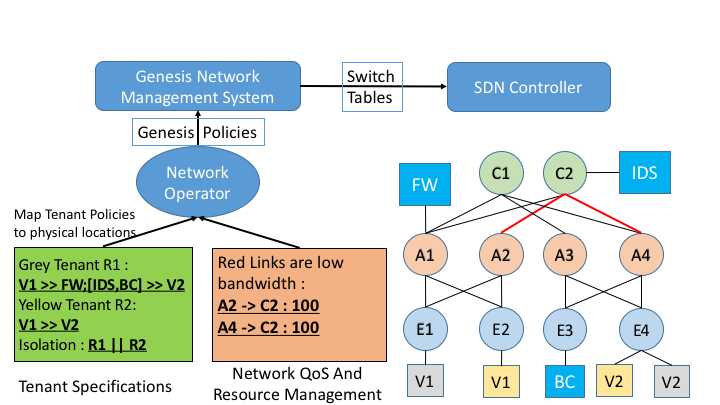
\includegraphics[height=7.5cm,right]{figures/architecture.png}
	\caption{Rough layout of system architecture. Also will come up with an example figure here.}
	\label{fig:architecture}
\end{figure}
In this section, we describe the type of policies that tenants and
network operators may wish to realize. %% For simplicity, we assume a
%% multi-tenant cloud set up, where both the tenants and the provider
%% wish to realize policies over their respective networks. However,
%% these policies, and our framework, are applicable to other settings,
%% e.g., enterprise networks with different departments imposing
%% different sets of policies.
We use Figure XXX as a running example. This figure shows several
tenants who differ in the nature of policies they wish to realize. We
note that these policies reflect and, in some cases, extend the
policies that enterprises realize in their on-site networks today as
well as policies that data center operators support for the different
workloads they host~\cite{mpa-imc15}.  The policies include:

\aditya{explain the figure here}.
\kausik{Will do this now}

\aditya{define flow, flow group, policy etc here}
% \aditya{need to start by saying we focus on multi-tenant clouds, although our system can apply elsewhere too}

% Operators of enterprise and multi-tenant clouds deal with policy
% requirements of different organisations and tenants, as well as
% require support to manage the network for providing QoS guarantees and
% network resource management internally, invisible to the
% tenants. Network operators need to be able to express complex policies
% in an intuitive declarative fashion, and the network management system
% must derive the individual switch forwarding behavior without
% involving the operator.


\begin{itemize}
\item \textbf{Reachability}: This enables network communication
  between specific groups of a tenant's virtual cloud instances,
  applications, or hosts. \aditya{refer here to an example in the
    figure}
\item \textbf{Middlebox traversals}: A tenant may wish that traffic
  between two of her endpoints, or from another tenant, must traverse
  through specific middleboxes (locations, or logical descriptors) for
  security, access control or performance reasons. This can be
  specified via an ordered sequence of sets of middleboxes for a flow
  group to traverse, where the middleboxes in a set can be traversed
  in any order, but all middleboxes in the set must be traversed.  The
  unordered set abstraction leverages the fact that middleboxes
  without dependencies in their traffic processing behavior can be
  placed in any order in a service chain~\cite{pga}. Thus the
  middlebox traversal specification outlined here generalizes the
  notion of a service chain.  \aditya{refer here to an example in the
    figure}

  %% \aditya{refer here to an example in
  %%   the figure} In several cases \loris{how true is this?} the order
  %% in which these middle-boxes is traversed is not relevant and the
  %% policy language should therefore support unordered waypoints.

\item \textbf{Isolation}: Tenants may require various QoS guarantees
  that enforce varying degrees of isolation for their traffic. In the
  extreme, a tenant could ensure that her flow groups are not affected
  by any other tenant by strictly isolating the path of the tenant's
  flows from others' flows. \aditya{refer here to an example in the
    figure} A tenant could also specify isolation for a subset of her
  (performance-sensitive) flows from other flows of her own deployment
  or those belonging to other tenants; the rest of the tenants' flows
  mayy require no guarantees.

%%   There has been a rising emergence of 
%% multi-tenant clouds, which is more economical for tenants to use
%% rather than managing their own private datacenters. However,
%% the current Service Level Agreements (SLAs)
%% provided to tenants are centered around compute, storage, or
%% external traffic bandwidth. Lack of guarantees on the network
%% between tenant instances leads to unpredictability of performance
%% for distributed applications. Also, multi-tenant clouds are
%% susceptible to attacks on the network by malicious tenants who could
%% hog the internal network bandwidth, or conduct side-channel
%% attacks~\cite{heyyou-ccs}.
% Conventionally,
% this problem is mitigated by static rate-limiting, but it can lead
% to under-utilisation of resources.
%% Cloud provider can offer (paying) tenants various QoS guarantees
%% that enforce varying degrees of tenant isolation. In the extreme,
%% this could ensure that a tenant's performance is not affected by
%% any other tenant by strictly isolating the path of tenant's flows
%% from others' flows. \aditya{refer here to an example in
%% 	the figure} The tenant could also specify isolation for certain
%%  performance-sensitive flows, while the rest of the tenant-flows
%%   would be without guarantees with varying degrees of pricing. 
%%   Thus, support for isolation is an important feature in multi-tenant 
%%   networks. 
 \end{itemize}
%TODO : MODIFY Synthesis of waypoints to support logical waypoints
%% Since, cloud tenants do not have a view of the actual physical
%% topology, the policy requirements for tenants are at a coarser level
%% of control. While support for the above policies can be used to satisfy tenant
%% SLAs, network operators can benefit from a fine-grained
%% control of network resources, integrated with support for tenant specifications 
%% for effective management of the network. \newline

\textbf{Network Resource Management}: While support for the above
policies can be used to satisfy tenant SLAs, network operators can
benefit from a fine-grained control of network resources, integrated
with support for tenant specifications for effective management of the
network. For instance, to aid traffic enginerring, the network
operator may specify policies constraining the maximum number of
tenant flows that can traverse a given link or sets of links in the
network. She may also wish to ensure traffic from some sensitive
applications does not contend for bandwidth on constrained links with
elastic traffic from batch applications.
          %% capacity
          %% of certain links such that tenant flows using the link do
          %% not exceed the capacity of the link. Such policies can be
          %% useful to ensure the low bandwidth links are not used by
          %% more tenants such that their performance is affected and
          %% can be used to provide bandwidth guarantees to tenants.
  Likewise, to tackle hardware heterogeniety, operators can specify
  switch constraint policies, like the size of the rule table to
  restrict the number of flows traversing a particular switch or set
  of switches.
%\item \textbf{Network Maintenance}: \aditya{this whole para does not
%    parse and needs updating} Operators on a regular basis perform link and
%  switch maintenances, and need to ensure that during maintenance, the network still
%  conforms to the SLAs of the tenants and resource capacity
%  policies.   \aditya{the following sentence does not make sense} Using Genesis, the operator
%  can specify the links and switches that will be down for maintenance, and Genesis can synthesize 
%  the rules for the updated network with all policies satisfies, which then can be pushed to 
%  the network before maintenance. 
%\end{itemize}

  Our goal is to design a system that allows the above policies to be
  specified in a simple, declarative manner, and abstracts away 
  data plane enforcement and the intricacies thereof.
  
\subsection{Synthesis} \label{sec:synthesis} 

\begin{table}[!t]
\begin{small}
	\begin{center}
		\begin{tabular}{m{7.8em}  m{15.9em} } 
			{\bf Policy} & {\bf Description} \\ 
			\hline
			Reachability & There is a path from router $src$ to router $dst$ for destination $\lambda$ \\ \hline
			Reachability with \newline Ordered Waypoints & The path  from $src$ to $dst$ for destination $\lambda$ 
			traverses some switch in the set $W_1$, \ldots, then some switch in the set $W_k$.\\ \hline
			Traffic Isolation & Paths of two reachability policies $R1$ and $R2$ do not share  links \\ \hline
			Traffic Engineering  & Minimize total/max link utilization \\
		\end{tabular}
	\end{center}
	\compactcaption{\genesis path-based policy support.} \label{tab:policysupport} 
\end{small}
\end{table}


%\section{Policy Support} \label{sec:policy}
%We design a language GPL (Genesis Policy Language) for network operators to express the desired end-to-end policies in a declarative manner which is interpreted by the Genesis synthesizer to find the forwarding rules for the network topology which enforce the input policies (\cref{fig:arch}). Genesis supports the following policies : 
%% Figure of GPL's syntax
%\begin{enumerate} 
%	\item \textbf{Reachability}: $predicate : src >> dst$ \\
%	This policy specifies the packets satisying $predicate$ have ingress router $src$ and egress router $dst$, and requires rules forwarding packets satisfying $predicate$ from $src$ to $dst$. There must be no forwarding loops in the network. 
%	\item \textbf{Waypoint}: $predicate : src >> W >> dst$ \\
%	The waypoint policy is a stronger reachability policy, and specifies that packet satisfying $predicate$ with ingress router $src$ and egress router $dst$ must pass through the set of waypoints $W$ in no particular order. The waypoint policy helps operators and tenants to specify the middleboxes the packets must traverse through without worrying about order, or having to use header tags to enforce a particular order \cite{flowtags}. 
%	\item \textbf{Traffic Isolation}:  $R1 \ || \ R2$ \\
%	The traffic isolation policy ensures that the . This policy can be used to provide fairness guarantees, since the paths of $R1$ and $R2$ don't share a link, the bandwidth used by $R1$ will not affect the bandwidth used by $R2$ and vice-versa. The condition of sharing a link in the same direction is due to the fact that links are full-duplex so, traffic flowing in one direction is not affected by the traffic flowing in the other direction.
%	\item \textbf{Security Isolation}: $R1 <> R2$ \\
%	The security isolation policy is stronger than the traffic isolation policy, and ensures that the path of the reachabiltiy/waypoint policies $R1$ and $R2$ do not share a link in both directions for increased security.
%	\item \textbf{}: $sw_1 \rightarrow sw_2 : capacity$ \\
%	The link capacity policy specifies that the capacity for link $sw_1 \rightarrow sw_2$ is $capacity$, and the weights of flows traversing the link in the direction of $sw_2$ do not exceed the capacity of the link.  
%	\item \textbf{Switch Table Size}: $sw : size$ \\
%	The router table size policy is used to specify the size of the forwarding table of the router $sw$ and ensures that the number of flows traversing through $sw$ does not exceed $size$ as each flow would require a forwarding rule at the switch.
%\end{enumerate}



Providing support for realizing the complex set of policies using
existing SDN programming languages like Pyretic and Frenetic is
challenging, because these policies are global and cannot be enforced
by programming individual behaviour of switches. Existing network
management systems provide support for complex policies including
middlebox placement and bandwidth constraints~\cite{}; however these
are tailor-made for certain policies and lack generality and
extensibility.

We design a general network management system that realizes the above
sets of policies by performing {\em synthesis} of switch forwarding
rules to enforce end-to-end policies. The system architecture of \name
is shown in \cref{fig:architecture} and the way in which policies
outlined in the previous section can be specified in \name is shown in
Table~\ref{tab:policysupport} .

Unlike previous efforts in the synthesis space (see~\cite{}), \Name is
not tailored to specific formalisms such as regular expressions and
this aspect makes it modular and easily extensible.
%and allows to devise specific
%techniques for each type of policies. 
To draw an analogy with SMT solvers, \Name can be seen as a constraint
solver that allows the addition different types of policies
(respectively, the theories in SMT) and that allows the design of
different types of optimizations based on the properties desired by cloud
  operators using \Name. 
  
Our work is motivated by recent progress in program synthesis.
Program synthesis is defined as the task of discovering an executable
program from user intent expressed in the form of some
constraints. There are three key dimensions to synthesis: the kind of
constraints that it accepts as expression of user intent, the space of
programs over which it searches, and the search technique it
employs. Program synthesis has seen limited applications to networks,
specifically to controller synthesis~\cite{netegg}, where the idea is
to learn from examples and synthesize the behavior of individual
switches (e.g., learning switches or firewalls); furthermore, this
technique applies to networks operating in a reactive mode (where the
first packet of a connection is processed by the controller to
determine the actions to employ). Like Frenetic~\cite{} and
Pyretic~\cite{}, this switch-centric approach is too constraining.

\Name\ leverages synthesis at a high level as follows: given a set of
policies which describe user intent, the search space is the space of
all forwarding plane configurations and the search technique involved
is SAT/SMT solving. The solution found is implemented by installing
the necessary switch rules via a skeleton controller.

This approach is appealing for a variety of different reasons: 

(1)
Policies useful to operators are \emph{proactive} (i.e., they are not
dependent on the actual packet flow), and our synthesis approach
naturally aligns with such proactive policies.

%  and this enables enforcing policies by synthesis
% of switch-table rules, and using a skeleton SDN controller to deploy
% the forwarding rules to the switches. In contrast, in trying to
% synthesize reactive policies (like a firewall), the controller needs
% to store the state of flows it has received and have a control module
% following the specifications \aditya{huh? this doesn't make sense...},
% which is an interesting synthesis problem, but orthogonal to our
% approach.

(2) Correct policy enforcement is challenging due to different
objectives for each of the policies - ensuring isolation between flows
may lead to overshooting capacity and vice-versa - and is a common
cause of incorrect configurations in networks.  Our approach removes
the need for a verification step in which the operator has to
``check'' whether an attempted configuration meets the desired
policies.  By using a formal reasoning technique, we are able to
consider the space of all forwarding configurations and find a
solution which is \emph{correct by construction}, i.e., it adheres to
satisfying a diverse set of policies, eliminating the room for error
by the network operator.

(3) Automatically enforcing policies is a task with
\emph{high theoretical complexity}. 
For example, enforcing isolation policies
is as hard as solving
graph-coloring, a well-known
NP-complete problem (see \cref{sec:isolationNP} for the proof).
%, which means
%that any system solving this would need to exhaustively search the
%space of all forwarding plane configurations. 
Many search techniques can be used to find the forwarding rules when
handling a particular class of policies, but when multiple types of
policies are combined (isolation, middlebox traversal, capacity
constraints), devising good search techniques becomes challenging.
Thanks to the many engineering efforts, SMT solvers abstract away most
of this complexity and allow us to unify the search objectives for
every policy into a generalized search technique.
%Thus, by reducing this problem to a SMT instance and
%leveraging fast off-the-shelf SMT solvers developed over years of
%research, \Name can provide support for diverse policies required by
%network operators. 
Crucially, \Name can be extended with ease to
support new policies without requiring changes to the search
techniques to find the solution.
%% \loris{I would like to convey that we are in some sense a Network solver module policy,
%% in the sense that we support theories (the policies) and now people can work on engineering
%% the solver for different classes of policies.
%% }
%% \kausik{To flow from this subsec to the next? Support for policies is 
%% 	inbuilt, but operators can engineer tactics to suit their needs. Is this what you want to convey?}
%% \loris{I found many words used to address the same concept:
%% enforce the policies, synthesize rules, etc...
%% try to be uniform or it's quite hard to understand what is being done.
%% } 
%% \kausik{I think "enforce policies" would be better? The title explains the rest.}

\subsection{Performance Challenges} \label{sec:performance}

One of the key challenges of \Name is the synthesis
performance. 
Due to the rich  policies supported by \Name
finding a consistent set of switch forwarding rules 
has exponential time worst case complexity in
the number of policies.
Moreover, since policies such as isolation affect
the paths many different flows, it is not possible to incrementally synthesize
the forwarding rules corresponding to each flow. 
Despite the recent advances in SMT solvers, to make
the synthesis problem feasible in practice,
there is a need to improve the performance of the solver
using techniques that are specific to the network domain.
\loris{I rewrote this previous paragraph}


In this paper, we propose various techniques leveraging
\emph{domain-specific} knowledge to improve synthesis performance. We
propose the idea of \emph{tactics} (\cref{sec:tactic}), which are
search strategies leveraging the network structure of datacenter
topologies, to specify properties of the paths for the reachability
policies.  Tactics are a way for network operators to specify a
high-level constraint on the set of paths allowed for reachability
policies.  Path properties are expressed using a simplified form of
regular expressions which, after being converted into a finite
automata, can be used to simplify the set of constraints provided to
the solver.  In particular, one can eliminate constraints that cannot
be true for any of the paths accepted by the automaton language. We
find that this can result in \aditya{XXX} speedup. \aditya{fill this
  in!} 


Another property of datacenter topologies is that the huge
interconnect of links can lead to multiple solutions to the problem
(i.e., to enforce the policies provided).  To take advantage of this
property, we design a heuristic procedure called \emph{optimistic}
synthesis (\cref{sec:optimistic}) which leverages the structure of
isolation policy interactions among tenants to partition the input
policies into effective components and synthesize these components
faster than the complete problem. To improve the effectiveness of the
heuristic, whenever the SMT solver fails to find a solution we extract
the unsatisfiability core produced by the SMT solver and 
add it to our set of constraints to quickly converge to a correct solution.
Informally, the unsatisfiability core can be viewed
as a set of constraints that describes why there wasn't a feasible solution~\cite{}. 
\loris{I rewrote this, should add a citation to something discussing unsat core}


\section{Synthesis Algorithm} \label{sec:synthesisalgo}
Given a set of policies, \Name creates constraints 
that abstract the forwarding and reachability rules such that the paths
satisfy the input policies.  
These constraints are then given to an SMT Solver, which returns a model 
for them--i.e., it assigns values to all the variables in the constraints. From these values, we extract the forwarding rules for each switch.
To provide support for the policies in \Cref{tab:policysupport}, \name uses propositional logic (SAT), linear rational arithmetic (LRA),
and linear optimization objectives for traffic engineering.
\subsection{Network Forwarding Model} \label{sec:fwdmodel}
We define the physical switch topology as an undirected graph $T=(S, L)$,
where $S$ is the set of switches and $L$ is the set of links. 
We use the neighbour function $N(s) = \{s'\ | \ (s,s') \in L \}$ to denote 
the set of neighbour switches of $s$. 
We define a set of packet classes $PC : [0,\lambda]$ and map each reachability/waypoint policy to a unique integer in $PC$.
The set of reachability policies is denoted as $R$ and each reachability policy $r \in R$ is
a pair
$(predicate :\newline src >> W_1;W_2; \ldots W_n >> dst, pc)$
where:
\begin{compactitemize}
\item  $predicate$ is the packet header identifier pertaining to $r$;
\item  $src,dst \in S$ are the source and destination switches;
\item $W_1, W_2, \ldots, W_n \subseteq S$ are the (potentially empty) ordered sets of waypoints; 
\item $pc \in PC$ is the packet class and is a unique integer used to identify the variables associated to $r$
\end{compactitemize} 
In the rest of the paper, we often use the term packet class to identify the corresponding reachability/waypoint policy. 
Other policies are not mapped to packet classes as they do not produce a path, but specify restrictions on paths of packet classes. 
%Assuming that the intersection of predicates is empty for policies in $R$, we create a mapping $\gamma : R \rightarrow PC$ to associate each reachability policy with a unique integer called packet class in the set $PC$. Switches $src, dst \in S$ denote the ingress and egress switches respectively for the packet class $pc = \gamma(r)$ and Genesis finds a path from $src$ to $dst$ for $pc$. If a waypoint policy is specified, $W$ is the set of switches the path from $src$ to $dst$ must traverse through in no particular order.
We define a static integer $\mu$ to be the synthetic limit for path length for any packet class, and define the set $K = [0, \mu]$ to be the set of all permissible path lengths.

The key roles of the network forwarding model are abstracting the actual forwarding rules at each node and encoding the reachability of each flow. 
\begin{mydef}
\label{def:fwd}
The relation $Fwd \subseteq S \times S \times PC $ captures network forwarding behavior, i.e. 
$(sw_1, sw_2$, $pc)\in$ $Fwd$ if 
$sw_1$ forwards packets of class $pc$ to switch $sw_2$. 
\end{mydef}
\begin{mydef}
\label{def:reach}
	The relation $Reach \subseteq S \times PC \times K$ captures the path reachability,
	i.e. $(sw, pc, k)\in Reach$ if 
	the switch $sw$ is reachable in the path from source switch of packet class $pc$ in exactly $k$ steps.  
\end{mydef}
For brevity, we write $Fwd(sw_1, sw_2, pc)$ for $(sw_1, sw_2, pc) $ $\in Fwd$ and similarly for the $Reach$ relation. 
Since $Fwd$ depends on the topology,
for all $sw_1, sw_2$ that are not connected by a link, 
we have that $\forall pc$, $(sw_1,sw_2,pc) \notin Fwd$. 
\begin{mydef}
	Given the set of constraints $\Psi$ generated by the synthesis algorithm from the input policies,
	$(Fwd,Reach) \models \Psi$ if $Fwd$ and $Reach$ is a model of $\Psi$.
\end{mydef}

\begin{mydef} \label{def:Pi}
Given two concrete relations $Fwd$ and $Reach$, 
the set of induced paths $\Pi = \texttt{paths}(Fwd, Reach)$ is defined as follows:
given a class $pc$,  $(sw_0 \ldots sw_k, pc) \in \Pi$ iff : 
\begin{compactenumerate}
	\item $\forall i \in [0,k]. (sw_i, pc, i) \in Reach$
	\item $\forall i \in [0, k - 1]. (sw_i, sw_{i+1}, pc) \in Fwd$
\end{compactenumerate}
\end{mydef}
\noindent Figure~\ref{fig:model} illustrates these definitions.

\begin{figure}
	\centering
	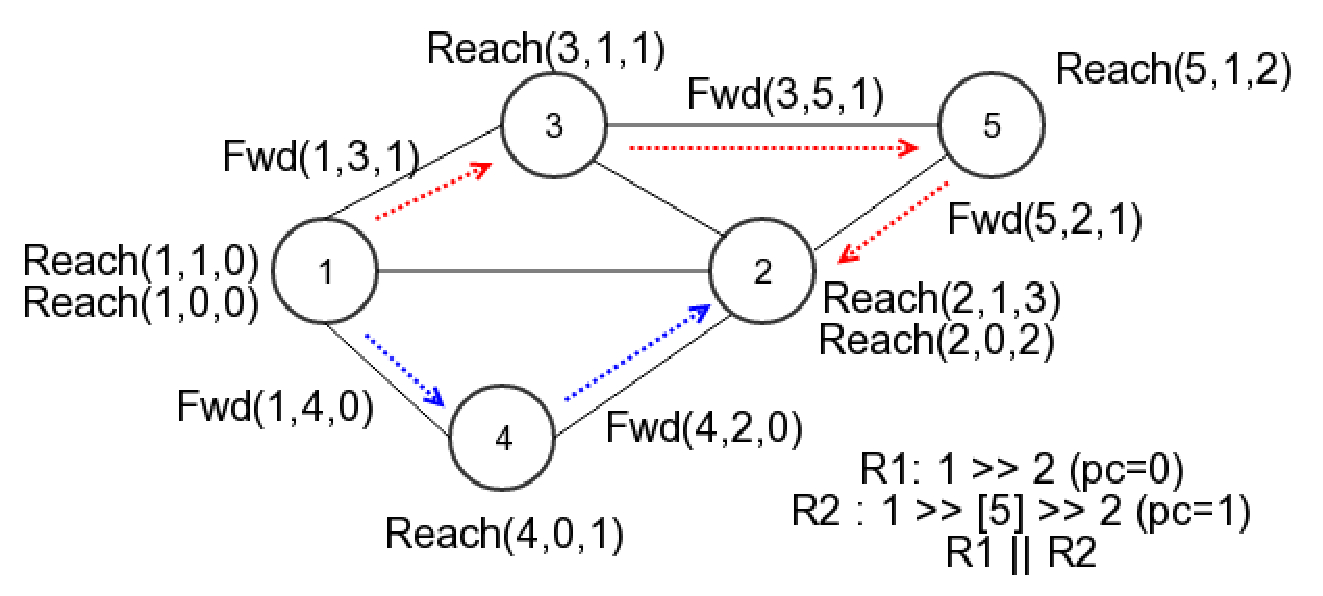
\includegraphics[width=0.8\columnwidth]{figures/network-model-example.eps}
	\caption{Values of the $Fwd$ and $Reach$ relations of the network forwarding model
		 for the policies specified in the figure. The blue and red arrows indicate the 
		 paths of packet classes 0 and 1 respectively according to the model.}
	\label{fig:model}
\end{figure}

\begin{mydef}
Given the set of constraints $\Psi$ corresponding to the input policies,
a set of paths $\Pi$ is a solution to $\Psi$, $\Pi \models \Psi$, 
if there exists $Fwd, Reach$ such that $(Fwd, Reach) \models \Psi$ and $\ \Pi=\texttt{paths}(Fwd,Reach)$.

\end{mydef}
%An example network forwarding model is shown in \cref{fig:model}. 
%%There are two reachability policies, $r1 : 1 >> [5] >> 2$ with $pc=1$ and $r2 : 1 >> 2$ with $pc=2$ and $r1$ is isolated to $r2$
%Using the value of $Fwd$ relation, we can find out paths for each packet class the forwarding rules for each switch. 

One of the decisions oriented towards performance is modelling the forwarding and reachability relations using propositions, so that we can reduce enforcement of policies like reachability, waypoints and isolation to a Boolean Satisfiability Problem (SAT) problem\footnote{An earlier iteration of our model used \emph{uninterpreted functions} and modeled reachability using recursive constraints, 
	which was slower with a greater number of constraints.}. 
The relations for forwarding and reachability ensure we can write the constraints in a concise and intuitive manner.

\subsection{Reachability Constraints} \label{sec:reach}
We first discuss the constraints generated for reachability policies without waypoints.
For a reachability policy $s >> d$ and packet class $pc$, the added constraints must ensure that 
the solution model represents a path 
from source to destination. 
The base constraint states that $(s, pc,0) \in Reach$ meaning
that $s$ can be reached in $0$ steps. 
The following constraint states that there must be a forwarding rule from $s$ to one of
the neighbors of $s$\footnote{
	We unroll the existential quantifier $\exists n \in N(s)$ using disjunction of 
	clauses $\bigvee\limits_{n \in N(s)}$ and
	the universal quantifier $\forall n \in N(dst)$ using conjunction of clauses $\bigwedge\limits_{n \in N(dst)}$
	and stay in propositional logic.}.
\begin{equation} \label{eq:src}
	\exists n \in N(s).~Fwd(s, n, pc) \wedge Reach(n, pc, 1).
\end{equation}
Next, we add the following constraints to state that $d$ can be reached in some number of steps and,
since $d$ is the last switch in the path, there are no forwarding rules from it.
\begin{equation} \label{eq:dst}
	\exists k.~Reach(d, pc, k) \ \wedge \ \forall n \in N(d). \ \neg Fwd(d, n, pc).
\end{equation}
Finally, we add implication constraints that propagate reachability backward from destination to source. 
If a node $n_1$ is reachable in $k$ steps, there must be a node $n_2$ reachable in  $k-1$ steps and 
a forwarding rule $n_2 \rightarrow n_1$.
\begin{multline} \label{eq:bckprop}
\forall n_1,k.~ Reach(n_1,pc,k) \implies \exists n_2.  n_2 \in N(n_1) \wedge \\ Reach(n_2,pc,k-1) \wedge Fwd(n_2,n_1,pc).
\end{multline} 
When combined together, these constraints %can only be satisfied if there is a valid path from $s$ to $d$.
% to destination by using the unit clauses in \cref{eq:dst}, and finding a path from destination back to a switch $sw$ which is a neighbour of $src$. $Reach(sw,pc,1)$ would be true from \cref{eq:src} and the reachability policy would be satisfied. 
are sufficient to ensure the existence of a path from $s$ to $d$ for packet class $pc$.
% in terms of the forwarding relation $Fwd$. 
However, since there is no restriction on number of $Fwd$ values that can be true at a switch, we can get multiple forwarding rules at switches, and 
also multiple paths to the destination. 
These can also create forwarding loops. 
Concretely, this is not a problem: as long as there is  at least one path from $s$ to $d$ we can recover it from the solution of the constraints. 
Moreover, this representation is quite efficient, as forcing a singular path would
require to add further constraints.
% we are able to extract a path from the solution without 
%adding additional constraints to ensure the semantics of \emph{unicast} forwarding. 

To extract a concrete $s$-to-$d$ path we 
perform a breadth-first search on the reachability graph induced by the solution to the constraints. 
A directed edge $n_1 \rightarrow n_2$ appears in the reachability-graph if there is forwarding rule indicated by the relation $(n_1,n_2, pc) \in Fwd$. 
We extract the rules relevant to the shortest path from source to destination from the model, and the additional rules obtained in the solution (extra paths, forwarding loops) are ignored.  

\subsection{Waypoint Constraints} 
For a reachability policy with ordered set of waypoints $s >> W_1;\ldots;W_n >> d$ and packet class $pc$, we add all the constraints specified in \secref{sec:reach} to ensure the existence of a path from $s$ to $d$. We then add constraints so that all waypoints $w$
are traversed. 
\begin{equation} \label{eq:waypoints}
	\forall w \in W_1, \ldots, W_n. \ \exists k.~Reach(w, pc, k).
\end{equation}
For each set $W_i$ for $i>1$, we add constraints to ensure that all waypoints
in $W_i$ are reached after all waypoints in $W_{i - 1}$ : 
\begin{multline}
\forall w_{i} \in W_{i}, \forall k_i.~Reach(w_i, pc, k_i) \implies 
\forall w_{i - 1} \in W_{i-1}. \\ \exists k_{i-1}. \ 
 k_{i-1} < k_{i} \wedge Reach(w_{i-1}, pc, k_{i-1}).
\end{multline}
%TODO
Previously, we imposed no restriction on the number of paths 
from $s$ to $d$. In the case of waypoints, this can result in 
a solution with multiple paths, with each individual path traversing
some of the waypoints, which is not the correct enforcement for a waypoint policy.
Thus, we need to ensure the solver returns a single path traversing
all the waypoints. To achieve this, we limit the number of
forwarding rules for $pc$ at a switch to 0 or 1. 
%%However, just ensuring reachability of waypoints is not sufficient. Since, we do not have any restrictions on the count of forwarding rules for a packet class at a switch, it is possible that waypoints are reachable from the source through separate paths, and do not lie in the path from source to destination. Thus, to ensure that all waypoints are reachable in the path from source to destination, we need to add constraints on the count of forwarding rules at each switch. 
%Forwarding rule constraints are to ensure that the forwarding relation $Fwd$ for a switch contains a \emph{single} switch which is a \emph{neighbour} or to no node at all (switches which are not reached in the path, and the destination will not have any forwarding rules). 
We define the forwarding set as:
\begin{equation}
	FwdSet(sw,pc) = \{k \ | \ Fwd(sw,k,pc)\}.
\end{equation}
We then add constraints stating that the size of the forwarding set must not exceed 1:
\begin{equation}
		\forall sw,pc .\ |FwdSet(sw,pc)| \leq 1 \label{eq:fwdset}.
\end{equation}
Here $|A|$ denotes the size of set $A$. The above constraints are expressed in SAT 
as follows: 
\begin{equation}
\bigvee_{\mathclap{k_1 \in N(sw)}} Fwd(sw, k_1, pc) \wedge (\bigwedge_{\mathclap{k_2 \in N(sw), k_2 \not= k_1}} \neg Fwd(sw, k_2, pc))
\end{equation}
%The forwarding set constraints ensure that the forwarding rules exist only on the path from source to destination, and no other rules exist in the solution. If a switch has a forwarding rule to  elsewhere, then it would not have a rule for the path, and the destination will not be reachable. These restrictions will also ensure there are no forwarding loops in the path. 
Since, there cannot exist multiple rules at a switch, the model will contain a 
single path from source to destination for $pc$ traversing the
waypoints in the right order.
%There would have to 
%be more than one rule at a switch for multiple paths from the source to exist. 

\subsection{Isolation Constraints}
A traffic isolation policy $pc_1 || \ pc_2$ states that the paths for
$pc_1$ and $pc_2$ do not share any link in the same direction.  We
enforce this policy by adding constraints that states that at every
switch, $pc_1$ and $pc_2$ must not forward to the same switch:
\begin{equation}
	\forall n_1.~\neg ( \exists n_2. Fwd(n_1,n_2,pc_1) \wedge Fwd(n_1,n_2,pc_2)). \label{eq:isolation}
\end{equation}
For a link isolation policy $pc_1 <> \ pc_2$ which prevents sharing a link
in both direction, the constraints added are:
\begin{multline}
\forall n_1.~\neg ( \exists n_2. Fwd(n_1,n_2,pc_1) ~~\wedge \\ (Fwd(n_1,n_2,pc_2) \vee Fwd(n_2,n_1,pc_2))). \label{eq:linkisolation}
\end{multline}
%These constraints are sufficient to ensure that the packet classes $pc_1$ and $pc_2$ would be isolated. 
When combined with \Cref{eq:fwdset}, these constraints guarantee
isolation
as there exists a single path for $pc_1$ and
$pc_2$ which would be isolated. 
Interestingly, for a reachability policy without waypoints,  
the constraints in \Cref{eq:fwdset} are not required to enforce isolation. 
Even though the solver could produce multiple forwarding rules which induce multiple paths, 
the constraints in \Cref{eq:isolation} or \Cref{eq:linkisolation} guarantee isolation as the solver would discard
the additional rules conflicting with another packet class.

%reachability policy. Thus, the solver would remove the additional rules which conflict with
%the other class while still ensuring a path exists from source to destination. 

%The isolation constraints is intuitive when coupled with the forwarding set constraints (\cref{eq:fwdset}) as the model only has forwarding rules for the path from source to destination. However, for a reachability policy without waypoints, we argue that the forwarding set constraints are not required when coupled with the isolation constraints. The reasoning behind this is that the solver would simply remove the extra forwarding rules of a packet class in the model which conflict with the other packet class, as there are no constraints which require the need of these extra forwarding rules for correctness, but are one particular solution model in the space of solutions. 

\subsection{Capacity Constraints} \label{sec:linkcap}
%%\subsubsection{Link Capacity Constraints} 
For a link capacity policy on the link $sw_1 \rightarrow sw_2: \omega$, 
we use the theory of linear rational arithmetic 
to add constraints on the link. As input, we have the traffic rates $\sigma(pc)$ of
each of packet classes, and the constraints must ensure that the traffic rate on $sw_1 \rightarrow sw_2$
does not exceed $\omega$ :
\begin{equation}
 \sum_{\forall pc} \texttt{ite}(Fwd(sw_1,sw_2, pc), \sigma(pc), 0) \leq \omega .
\end{equation}
If a class $pc$ uses link $sw_1 \rightarrow sw_2$, then $(sw_1,sw_2, pc) \in Fwd$
and $\sigma(pc)$ is added in the utilization of the link. \\
\noindent A switch table policy $sw : \gamma$ specifies that the number of forwarding 
rules on $sw$ must not exceed $\gamma$. Similar to the link capacity policy,
the constraints ensure the count of all packet classes which traverse $sw$ (each 
will require a forwarding rule) is $\leq \gamma$ :
\begin{equation}
\sum_{\forall pc} \texttt{ite}(~\exists k. Reach(sw,pc,k), 1, 0)  \leq \gamma.
\end{equation}

%In terms of our model, the link capacity policy translates to constraints that
%ensure that the tuples of the form $(sw_1, sw_2, pc) \in Fwd$ for $pc \in PC$ conform to the capacity specified in the policy, 
%as the forwarding rule $sw_1 \rightarrow sw_2$ means that the link is being used by the particular packet class.
% 
%Let $C(sw_1,sw_2,pc)$ be the cumulative capacity function of the link used by all packet classes less than equal to $pc$. Since we use integers for denoting the packet class, we have a total order of the set of packet classes. We use this to create inductive constraints to sum over the set of Boolean variables $Fwd(sw_1, sw_2,pc)$. Let $PC : [0, \lambda]$ be the set of packet classes and $W(pc)$ 
%denote the capacity of packet class $pc$--i.e., the bandwidth allotted to the packet class. 
%The base case constraint for the capacity function is for $pc = 0$:
%\begin{multline}
%\neg Fwd(sw_1, sw_2, 0) \implies C(sw_1, sw_2, 0) = 0 \\
%	Fwd(sw_1, sw_2, 0) \implies C(sw_1, sw_2, 0) = W(0)
%\end{multline} 
%If link is used, the inductive constraints for the capacity function are as follows:
%\begin{multline}
%	\forall pc > 0.~Fwd(sw_1,sw_2,pc) \implies \\ C(sw_1, sw_2, pc) =  C(sw_1, sw_2, pc - 1) + W(pc)
%\end{multline}
%If the link is not used, the constraints are as follows : 
%\begin{multline}
%\forall pc > 0.~\neg Fwd(sw_1,sw_2,pc) \implies \\ C(sw_1, sw_2, pc) =  C(sw_1, sw_2, pc - 1)
%\end{multline}
%To satisfy the policy, the total capacity used should not exceed $\omega$. 
%Since $\lambda$ is the greatest element in $PC$ we have:
%\begin{equation}
%	C(sw_1, sw_2, \lambda) \leq \omega
%\end{equation} 
%For \emph{switch table size} policies, we need to track the number of packet classes that traverses the switch.
%We create inductive constraints similar to those for link capacity.
%. for counting the packet classes traversing $sw$.

\section{Synthesis with Optimization Objectives}
We describe two applications paramount to network management:
traffic engineering and network repair, which can be tackled using
extensions of solvers: SMT with linear optimization objectives and MaxSMT ~\cite{}.
\subsection{Traffic Engineering}
While the link capacity policies described in \Cref{sec:linkcap} can
be used to perform a strict form of traffic engineering in terms of 
adhering to link bandwidths, support for traffic engineering objectives
like minimizing the max link utilization, minimizing average link utilization
is highly \emph{desirable}. By specifying linear optimization objectives over
SMT formulas, \name can synthesize paths satisfying policies and minimizing
a global traffic engineering objective. 

To perform traffic engineering, link capacities of the network $C(sw_1, sw_2)$ and traffic 
rates of the packet classes $T(pc)$ are specified as input to \name (we assume a single
path for a packet class). The utilization 
of a link $U(sw_1, sw_2)$ is defined as the ratio of total traffic flowing through the link to the 
link capacity, and encoded in Z3 using the theory of rational linear arithmetic as:
\begin{equation}
U(sw_1, sw_2) = \frac{\sum_{\forall pc} \texttt{ite}(Fwd(sw_1,sw_2, pc), T(pc), 0)} {C(sw_1, sw_2)}
\end{equation}
The TE objective of minimizing average link utilization is equivalent to minimizing
the total link utilization (as average = total/constant). Thus, the minimization
objective is:
\begin{equation}
	\texttt{minimize}\ \sum_{\forall sw_1, sw_2} U(sw_1, sw_2)
\end{equation}
To encode the TE objective of minimizing the maximum link utilization, we define
a variable $maxU$, and constraints to ensure that $maxU$ is greater than or equal to all 
individual link utilisations, and the objective: 
\begin{equation} \label{eq:maxu}
\forall sw_1, sw_2.\ \ maxU \geq U(sw_1, sw_2)
\end{equation} 
\begin{equation}
		\texttt{minimize}\ maxU
\end{equation}
While $maxU$ can be set to a large value trivially to satisfy \Cref{eq:maxu}
, since the objective is to minimize $maxU$, it will be set to the actual
minimized maximum link utilization. Using an encoding similar to the one presented in this section, \name can be used for other objectives like minimizing total latency and load balancing
traffic across the network middleboxes.

\subsection{Network Repair}
While policy-compliance is a major requirement in a network management system,
another important consideration is datacenters is the occurence of failures (switches, links etc.),
which requires recomputation of paths compliant to the policies for the modified topology. 
Also, the network requirements are constantly \emph{in flux}, and operators have the requirement to 
add new tenants/policies. While a naive approach is to use \name to resynthesize the modified instance,
the new solution may be drastically different from the original configuration, incurring a
large overhead of changing the forwarding rules. This can also be used to
port existing non-policy compliant configurations deployed in a network to
satisfy a set of policies.

We extend \name's synthesis algorithm for performing
minimal network repair using MaxSMT.  
Formally, the weighted MaxSMT problem is as follows: given a set
of formulas $\Psi_0, \Psi_1, \ldots \Psi_n$ with associated 
weights $w_1, \ldots w_n$, find a subset $M \subseteq \{1, \ldots n\}$
such that 
\begin{enumerate}
	\item $\Psi_0 \wedge \bigwedge_{i \in M} \Psi_i$ is satisfiable.
	\item The \emph{award} $\sum_{i \in M} w_i$  is maximized.
\end{enumerate}
The constraints $\Psi_1, \ldots \Psi_n$ denote \emph{soft} constraints, and
the weights $w_i$ encodes the award for including $\Psi_i$ in the satisfying
assignment. 
%The basic intuition is that
%we add the existing configuration as \emph{soft} constraints to the set of \emph{hard} 
%policy constraints. The solver would return a solution which \emph{maximizes} the 
%number of satisfied soft constraints (the older configuration),
%thus resulting in a new policy-compliant forwarding 
%configuration with minimal 
%number of changes from the older one and reducing the overhead of
%updating the forwarding rules in the network.  

Network repair is reduced to a MaxSMT problem
such that \name minimizes
the number of switches on which rules needs to be updated. Let
the policy constraints generated by \name be $\Psi_0$, and the present 
configuration is $(\overline{Fwd})$ which does not satisfy $\Psi_0$. The 
objective is to find new $Fwd$ which satisfies $\Psi_0$ such that the number of \emph{unaffected} switches 
is maximized.If a switch $sw_i$ is unaffected, then $Fwd$ and $\overline{Fwd}$
has the same forwarding rules: 
\begin{equation}
	\Psi_i =  
	  \bigvee_{\mathclap{\substack{\forall sw_j, pc \\
			  		(sw_i, sw_j, pc) \in \overline{Fwd}}}} Fwd(sw_i, sw_j, pc) 
			~~~~~~~~~~~ 
			w_i = 1
\end{equation}
With $\Psi_0, \Psi_1, \ldots \Psi_n$ and associated weights $w_1, \ldots w_n$
to a MaxSMT solver, we can synthesize a new forwarding configuration 
which \emph{minimizes} the number of switches which have to be changed.
The weights can be altered for different priorities for different switches. Alternate
repair objectives like minimizing number of changed forwarding rules (instead of 
switches) can also be expressed as a MaxSMT problem. 

%\name is provided the policies
%and the current forwarding rules $(\overline{Fwd})$ as input. The policy constraints are added as hard
%constraints as described in the earlier sections. To maximize the number of unchanged
%switches, we add \emph{soft} constraints for each switch $sw_1$ of uniform weight as follows:
%Thus, the new forwarding rules $Fwd$ will maximise the number of unchanged
%switch rules in $\overline{Fwd}$, because the constraint will be unsatisfied if a rule on the
%switch changes. 


 







 
\subsection{Handling Failures Gracefully}

Another network management consideration for operators is the
occurence of failures (switches, links etc.), which are all too
frequent in datacenter networks~\cite{datacenterfailures}. Failures require
recomputation of paths compliant to the input policies
for the modified topology.  A naive approach is to use \name to
resynthesize the modified instance; However, the new solution may be
drastically different from the original data plane, incurring a large
overhead of removing old rules and installing new
ones~\cite{sdnlatency,updatescheduling}. 
%which could lead to serious
%disruption of tenants' flows.


In what follows, we describe two techniques to handle failures more
gracefully. The first technique is data-plane resiliency (\secref{sec:resiliency}),
which synthesizes and
pre-installs resilient data planes, which even in the event of a
bounded number of link failures, continue to satisfy input
policies. This technique eliminates the need to resynthesize the
forwarding rules for every network failure event, but it 
requires extra backup rules on switches, and it also cannot
capture global operator policies.

Thus, we propose a second mechanism called \emph{minimal repair} (\secref{sec:repair}),
which can transition from the disrupted data
plane to a new policy-compliant one with minimal overhead
 by minimizing the number of
switches whose rule tables are modified. 
Repair does not incur the extra rule cost of the first approach 
and can capture all \Name policies. It is also useful for 
accommodating incremental policy changes, which occur frequently in
cloud datacenters~\cite{mpa-imc15}. The main drawback is that it still
requires removal/installation of rules when a failure occurs, which
can end up being expensive depending on the number of switches
involved.

%% Although the minimal repair mechanism

%% The minimal repair mechanism has two drawbacks: (1) It is {\em reactive}. (2) MaxSMT can be slow to compute a solution impose a high delay to respond to a failure. 
%% cases impose an undue {\em time} overhead in transitioning to the new
%% dataplane.
%% For the new set of policies,
%% \name can use repair to synthesize a new data plane with minimal
%% overhead of installation.



%\name is provided the policies
%and the current forwarding rules $(\overline{Fwd})$ as input. The policy constraints are added as hard
%constraints as described in the earlier sections. To maximize the number of unchanged
%switches, we add \emph{soft} constraints for each switch $sw_1$ of uniform weight as follows:
%Thus, the new forwarding rules $Fwd$ will maximise the number of unchanged
%switch rules in $\overline{Fwd}$, because the constraint will be unsatisfied if a rule on the
%switch changes. 


\subsubsection{Dataplane Resiliency}
\label{sec:resiliency}

%% , and it is crucial to provide
%% certain guarantees during failure scenarios. For example, if the
%% operator wants to guarantee reachability amongst a pair of endpoints,
%% the controller only has to find an active path in the network to
%% re-establish reachability.  However, upon the failure of a link, {\em
%%   reactively} synthesizing a new data plane which satisfies all input
%% policies can be time-consuming, and during this period multiple
%% tenants can suffer from lack of reachability and/or performance
%% issues.  Thus, we propose \emph{policy-compliant resiliency} to tackle
%% network failures by \emph{proactively} synthesizing resilient data
%% planes that even in the event of a bounded number of link failures,
%% continue to satisfy input policies. This eliminates the need to
%% resynthesize the forwarding rules for every network failure event.

In this section, we describe the transformation of input policies to
provide dataplane \emph{t-resilience}~\cite{plinko}, i.e., in the event of
upto $t$ arbitrary link failures, the synthesized data plane still has
a path for each packet class satisfying all policies which is achieved
by synthesizing backup paths that satisfy input policies.  We only
consider reachability, waypoint, and isolation policies in the input.
Global policies like capacity policies and traffic engineering pose a
difficulty in synthesis. For example, consider a packet class $pc$
with a traffic rate of $\sigma(pc)$. By considering the backup paths
with the same traffic characteristics for synthesis, the total traffic
accounted for $pc$ would be $c\times \sigma(pc)$ (for some constant
$c$), leading to under-provisioning of resources. Our current
resilience transformation has no provisions to avoid or minimize the
under-provisioning of resources which affect capacity policies and TE
objectives.
%all backup paths in consideration, while all backup paths will not 
%exist together in the network (backup paths will be deployed during
%a failure event).
%\loris{don't understand previous sentence} \kausik{Have to think!}

Given the physical topology $T=(S,L)$, we define a link-failure
scenario $\theta$ as the set of failed links such that $\theta \subseteq L$.
% For \emph{t-resilience}, we need to
%consider synthesis under any set of $t$ or less arbitrary link failures.
%\begin{mydef}
	We define $\Theta(t)$ as the set of all failure scenarios where no more than $t$
	arbitrary links fail,---i.e. $\Theta(t) = \{ \ \theta \ \ | \ \ |\theta| \leq t\}$.
%\end{mydef}
%We define the projected topology $T^{\theta} = (S, L - \theta)$ as the active 
%physical topology under the failure scenario $\theta$. 	For each class $pc$,
%we construct a data plane graph $\xi = (S, L_{pc})$ for packet class $pc$ from the set
%of paths obtained from the synthesis algorithm. $\xi$
%for class $pc$ over a projected topology $T^\theta$ 
%is resilient if the graph $(S, L_{pc} - \theta)$ has a path from $src$ to $dst$ 
%for the packet class. 
Given a packet class $pc$,
we construct the induced data plane graph $\xi = (S, L_{pc})$ from the links
of the paths returned by the synthesis algorithm for class $pc$.
 For a failure scenario
$\theta$, the active data plane $\xi_\theta = (S, L_{pc} \setminus \theta)$ represents
all the links used by $\xi$ which are unaffected by the failure scenario. A data
plane $\xi$ is {\em resilient} to $\theta$ if it contains a path from the source to 
destination for the packet class in the active data plane $\xi_\theta$.
\begin{mydef}[Resilience]
	A data plane $\xi = (S, L_{pc})$ for class $pc$ is t-resilient if $\xi$ is 
	resilient to all $\theta \in \Theta(t)$.
\end{mydef}
While resilience deals with 
existence of paths during failure scenarios,
we extend the notion to include policy compliance.
\begin{mydef}[Policy-compliance]
	A t-resilient data plane $\xi = (S, L_{pc})$ for class $pc$ is policy-complaint if under
	any failure scenario $\theta \in \Theta(t)$, any path for $pc$ in 
	$\xi_\theta=(S, L_{pc} \setminus \theta)$ satisfies the input policies. 
\end{mydef}
\begin{algorithm}[h]
	\begin{footnotesize}
		\caption{Resilience Transformation}
		\label{restransform}
		\begin{algorithmic}[1]
			\State{[Input] $PC$: Packet classes (Reachability/Waypoint policies)}
			\State{[Input] $I$: Isolation policies (Traffic and Link types)}
			\State{[Input] $t$: Maximum number of arbitrary link failures}
			\State{[Output] $PC^R, I^R$: Transformed set of policies such that the synthesized data
				plane is \emph{t-resilient} and policy-compliant}
			\vspace*{0.25cm}
			\State{$PC^R, I^R \leftarrow \emptyset$}
			\For{$pc:\{src_{pc},dst_{pc},W_{pc}\} \in PC$} 
			\State{// Create $t+1$ edge-disjoint paths of $pc$}
			\State{$\hat{pc} = \{rc_1, rc_2, \ldots rc_{t+1}$\} s.t $\forall m. \ rc_m: \{src_{pc},dst_{pc},W_{pc}\}$} \label{lst:line:respc}
			\State{$PC^R = PC^R \cup \hat{pc}$} 
			\State{$I_{pc} = \{rc_m <> rc_n\ |\ \forall m,n \leq t+1 \wedge m < n\}$}  \label{lst:line:respcisolate}
			\State{$I^R = I^R \cup I_{pc}$} \label{lst:line:respcend}
			\EndFor
			\For{$i: pc_m <op> pc_n \in I$} 
			\State{$\hat{i} = \{ rc_1 <op> rc_2\ | \ \forall rc_1 \in \hat{pc_m}, \forall rc_2 \in \hat{pc_n} \}$} \label{lst:line:respolicy}
			\State{$I^R = I^R \cup \hat{i} $}
			\EndFor \\
			\Return{$PC^R, I^R$}
		\end{algorithmic}
	\end{footnotesize}
\end{algorithm}

\Cref{restransform} shows how \Name can be used to provide \emph{t-resilience}.
The idea is to modify the input policies such that multiple disjoint paths satisfying the original
policies are synthesized for each packet class. 
For \emph{t-resilience}, a packet class $pc$ needs at least $t+1$ edge-disjoint paths from
source to destination. 
We ensure this property holds by creating 
$t+1$ new packet classes ($\hat{pc}$ in line~\ref{lst:line:respc})
and use {\em link-isolation policies} amongst all pairs in $\hat{pc}$ (line \ref{lst:line:respcisolate})
to create $t+1$ edge-disjoint paths for $pc$.
The synthesized data plane $\hat{\xi} = (S, L_{pc})$ for class $pc$ is constructed from the 
paths in the resilient packet class set $\hat{pc} = \{rc_1,\ldots,rc_{t+1}\}$,
i.e., $L_{pc} = \bigcup\limits_{rc \in \hat{pc}} L_{rc}$.  
Each path of $\hat{pc}$ satisfies the reachability policy, 
and any arbitrary $t$ link failure scenario cannot affect all $t+1$ paths.

However, the resilient paths need to satisfy the input isolation policies with other 
packet classes (which themselves have $t+1$ paths for resilience). Thus, for a 
given policy $pc_1 || ~pc_2$, we add isolation policies to every pair of 
classes of $\hat{pc_1}$ and $\hat{pc_2}$ (line \ref{lst:line:respolicy}). This ensures that any path 
chosen in the data planes of $pc_1$ and $pc_2$ will be isolated from one 
another, thus providing policy-compliance under any arbitrary $t-link$ failure
scenario. \Cref{fig:restransform}(a) demonstrates an example transformation for providing $1-resilience$. 

\noindent We now that \Cref{restransform} is sound.
\begin{theorem}[Soundness]
Given input policies $(PC, I)$, 
the data plane $\hat{\xi}_{pc}$ for every packet class $pc \in PC$
 synthesized from
transformed policies $(PC^R, I^R)$  is \emph{t-resilient} 
	and policy-compliant. 
\end{theorem}
\iffull
\begin{proof}
		Assume, $\exists pc$ such that the data plane $\hat{\xi} = (S, L_{pc})$
		is not \emph{t-resilient}. 
		Therefore, there exists a failure scenario $\theta$ such that $|\theta| \leq t$ 
		and $\hat{\xi}_\theta = (S, L_{pc} \setminus \theta)$ 
		is not resilient, i.e., there is no path from the source to destination. 
		Thus, $\theta$ disabled all the paths of $\hat{pc}$. \\
		However, the paths are
		edge-disjoint as each class in $\hat{pc}$ has a link-isolation policy with each 
		other. Thus, $t$ link failures cannot affect $t+1$ 
		edge-disjoint paths of $\hat{pc}$. Thus, $\theta$ disabling all paths of
		$\hat{pc}$ is a contradiction. \\
		Let us consider policy-compliance. Given a failure scenario $\theta \in \Theta(t)$, each data plane $\xi$ of class $pc$ has an active path. Consider a isolation policy in $I$: $pc_1 || \ pc_2$. In line~\ref{lst:line:respolicy} of \Cref{restransform}, each class of $\hat{pc_1}$ will be isolated to
		each class of $\hat{pc_2}$, thus any path of the data planes of $pc_1$ and
		$pc_2$ will satisfy the input policy $pc_1 || \ pc_2$. Hence, the data planes 
		are policy-compliant. 
	\end{proof}
	\fi
\noindent If there are no isolation policies in the input, the resilience transformation in lines 
\ref{lst:line:respc}-\ref{lst:line:respcend} of \Cref{restransform} is complete.
\begin{theorem}[Completeness]
%\loris{What is the input? You should say.
%Given .... such that ...., the synthesized data plane... is....if and only if...}
Given input policies $(PC,I)$ such that $I=\emptyset$,
the synthesized data plane $\xi$ for a packet class $pc$  
is \emph{t-resilient} if and only if it 
contains $t + 1$ edge-disjoint paths from source to destination
for $pc$.
%If there are no isolation policies $I = \emptyset$, 
%	for a packet classes $pc$, the data plane \loris{what dataplane?} is \emph{t-resilient} only if it 
%	contains $t + 1$ edge-disjoint paths for $pc$.
\end{theorem}
\iffull
	\begin{proof}
		We have proved the soundness of the result in \Cref{resiliencesoundness}. 
		Now, let us assume the data-plane $\hat{\xi}$ for $pc$ is \emph{t-resilient} such 
		that less than $t+1$ instances of $pc$ are required for resilience i.e. 
		$|\hat{pc}| < t+1$. Let us consider a 
		t-link failure scenario $\theta, |\theta| = t$ where a link is picked from
		each path of $\hat{pc}$. The active data plane
		$\hat{\xi}_\theta = (S, L_{pc} \setminus \theta)$ will not contain a
		path from source to destination as all paths of $\hat{pc}$ would be disabled.  
		This is a contradiction since $\hat{\xi}$ is \emph{t-resilient}. 
		Therefore, we need atleast $t+1$ instances of $pc$ to ensure \emph{t-resilience}.
		
		Now let us assume there are $t+1$ paths in a \emph{t-resilient} $\hat{\xi}$ for $pc$,
		and not all of them are edge-disjoint. Consider two paths $\pi_1$ and $\pi_2$
		in $\hat{\xi}$ which share a link. We can choose the shared link 
		of $\pi_1$ and $\pi_2$ and $t-1$ links from the other $t-1$ paths 
		and construct a failure scenario $\theta$, $|\theta| = t$.
		The active data plane
		$\hat{\xi}_\theta = (S, L_{pc} \setminus \theta)$ will not contain a
		path from source to destination as all paths of $\hat{pc}$ would be disabled.  
		This is a contradiction since $\xi$ is \emph{t-resilient}. Therefore,
		the $t+1$ paths of $pc$ must be edge-disjoint. 
		
		\noindent Thus, the resilience transformation is sound and complete for a  
		packet class if there are no isolation policies.
	\end{proof}
\fi

%\noindent The transformation demonstrated in \Cref{restransform} is not \emph{complete}
% if the original policies contain link-isolation policies i.e. if the transformed policies
% are unsatisfiable, 
% that does not imply the non-existence of resilient data planes. 
When the original policies contain link-isolation policies, the policies
from \Cref{restransform} may return \texttt{unsat} even when a
resilient data plane exists. Specifically, line~\ref{lst:line:respolicy}
can add additional policies than is required for resilience.
% This is because link-isolation causes edge-disjointness of paths,
% and thus, cannot be both affected by a link failure. 
 \Cref{fig:restransform}(b) shows a transformation required for $1-resilience$ 
 with a smaller number of link-isolation policies among different classes
 of $pc_1$ and $pc_2$ than one obtained from \Cref{restransform}. 
 Consider a failure scenario which disables path
 of $pc_{1A}$. By virtue of the link-isolation policies, $pc_{1B}$ and
 $pc_{2A}$ will be unaffected and can be used as paths for $pc_1$ 
 and $pc_2$ respectively, and $pc_1 <> pc_2$ holds. Now suppose
 $pc_{1B}$ is affected. Similarily, $pc_{1A}$ and $pc_{2A}$ can be used as
 the paths for the original packet classes. The same scenarios hold symmetrically
 for $pc_2$, and thus the resilience transformation can be achieved without
 adding link-isolation policies amongst all the packet classes. 
 
\begin{figure}
	\centering
	\subfloat[Traffic Isolation]{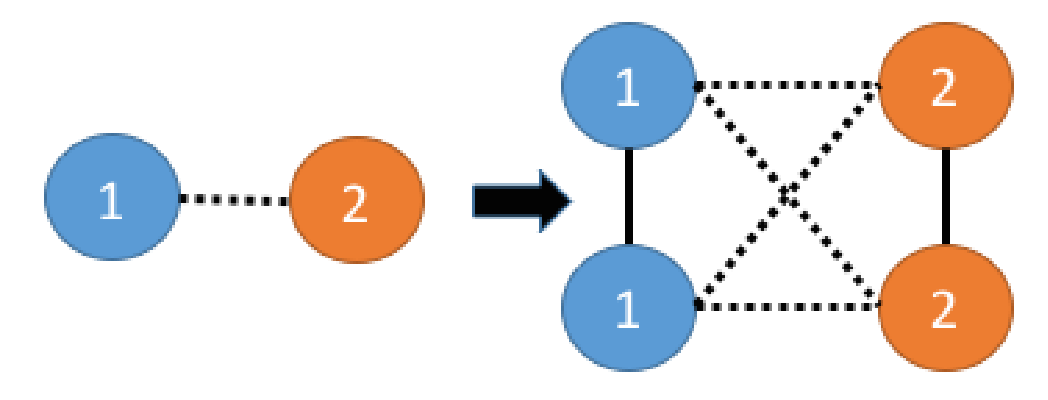
\includegraphics[width=0.5\columnwidth]{figures/resilience.eps}}
	\subfloat[Link Isolation]{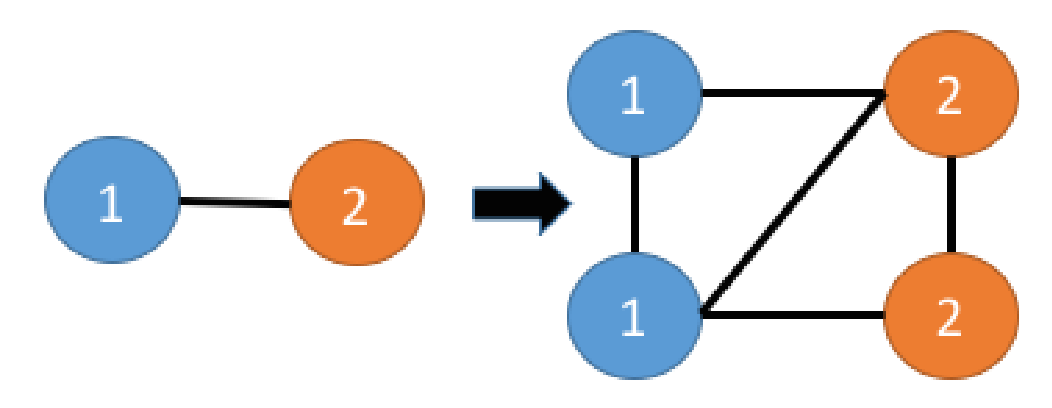
\includegraphics[width=0.5\columnwidth]{figures/resilience-cex.eps}}
	\caption{\label{fig:restransform}
		(a) Resilience Transformation for $pc_1 || \ pc_2$ for providing $1-resilience$. 
		The dotted lines represent traffic isolation policies, 
		while the solid lines represent link isolation. (b) Example of a sufficient transformation
		for 1-resilience in the case of a link-isolation policy.}
\end{figure}

%We presented a sound transformation of policies to provide \emph{t-resilience} in
%the case of reachability, waypoint and isolation policies. Future directions of 
%research involve incorporating capacity constraints and traffic engineering
%for synthesis of resilient data planes and devising a complete transformation for isolation.

\subsubsection{Minimal Repair} \label{sec:repair}
%% Thus, operators need
%% a \emph{network repair} mechanism which can transition with minimal
%% overhead from the current data plane to a policy-compliant one.  This
%% repair mechanism is also useful to accomodate incremental policy
%% changes, which occurs frequently in cloud
%% datacenters~\cite{mpa-imc15}.  For the new set of policies, \name can
%% use repair to synthesize a new data plane with minimal overhead of
%% installation.

Dataplane resiliency imposes high rule storage overhead on switches,
and cannot accommodate global policies like link capacity bounds. 
As an alternative to it, we
extend \name's synthesis algorithm to perform minimal network
repair using MaxSMT.

Formally, the MaxSMT problem is as follows:
given a set of formulas $\Psi_0, \Psi_1, \ldots, \Psi_n$ with
associated weights $w_1, \ldots, w_n$, find a subset $M \subseteq \{1,
\ldots n\}$ s.t:
1) $\Psi_0 \wedge \bigwedge_{i \in M} \Psi_i$ is satisfiable, and 
2) The \emph{award} $\sum_{i \in M} w_i$  is maximized. 
The constraints $\Psi_1, \ldots, \Psi_n$ denote \emph{soft} constraints, and
the associated weights $w_i$ encode the award for including $\Psi_i$ in the satisfying
assignment. 
%The basic intuition is that
%we add the existing configuration as \emph{soft} constraints to the set of \emph{hard} 
%policy constraints. The solver would return a solution which \emph{maximizes} the 
%number of satisfied soft constraints (the older configuration),
%thus resulting in a new policy-compliant forwarding 
%configuration with minimal 
%number of changes from the older one and reducing the overhead of
%updating the forwarding rules in the network.  

We reduce the network repair problem to a MaxSMT problem
and use soft constraints to minimize the number of 
switches on which rules need to be updated. Note that
the disadvantage w.r.t. dataplane resiliency is that switches still
require rule updates, which may take time depending on the number of
switches involved.

 Let the policy constraints generated by \name for the new network
 state be $\Psi_0$, and let $\overline{Fwd}$ be the present data plane
 that does not satisfy $\Psi_0$. The objective is to find new $Fwd$
 which satisfies $\Psi_0$ while maximizing the number of \emph{preserved
   switches} (switches whose rules are unchanged). If the
 rules on switch $sw_i$ are preserved, then $Fwd$ and $\overline{Fwd}$
 have the same forwarding rules for all packet classes which traverse
 through $sw_i$. The following soft constraints capture this idea:
\begin{equation}
	\Psi_{sw_i} =  
	  \bigvee_{\mathclap{\substack{\forall sw_j, pc \\
			  		(sw_i, sw_j, pc) \in \overline{Fwd}}}} Fwd(sw_i, sw_j, pc) 
			~~~~~~~~~~~ 
			w_{sw_i}= 1
\end{equation}
The solution to this MaxSMT problem is a data plane that minimizes the number of
switches whose rules have to be changed.  Alternate repair objectives
like minimizing the number of changed forwarding rules can be
expressed similarly. Interestingly, the \name's network repair
mechanism can also be used to transform an existing
non-compliant data plane to a policy-compliant one.

%- in some cases search is still hard but the network operator might have an idea of what the path patterns might or might not look like - Done
%- example? - Done
%- a good way to express this is to add extra constraints of the form ... - Done
%- we formally define a subset of regexes that...?
%- algorithm
%- brief comparison with netgen
\section{Tactics} \label{sec:tactic}
Synthesizing a data plane translates to choosing paths from
the solution space of all paths for each reachability policy such
that the chosen paths satisfy all policies, e.g., waypoint traversal
and isolation. Datacenter topologies, e.g., fat-trees~\cite{fattree},
have numerous paths between edge switches to provide full bisection
bandwidth.  Thus, the solution space of paths for a pair of endpoints
is large.  For example, consider the fat-tree topology in
\Cref{fig:fattree}.  The number of paths under length 10 between two
edge switches in the same pod is 242 and between two edge switches in
different pods is 272.  If we consider the synthesis of $n$ packet
classes, the problem roughly translates to finding a solution in the
space of size $(242)^n$.
\begin{figure}
	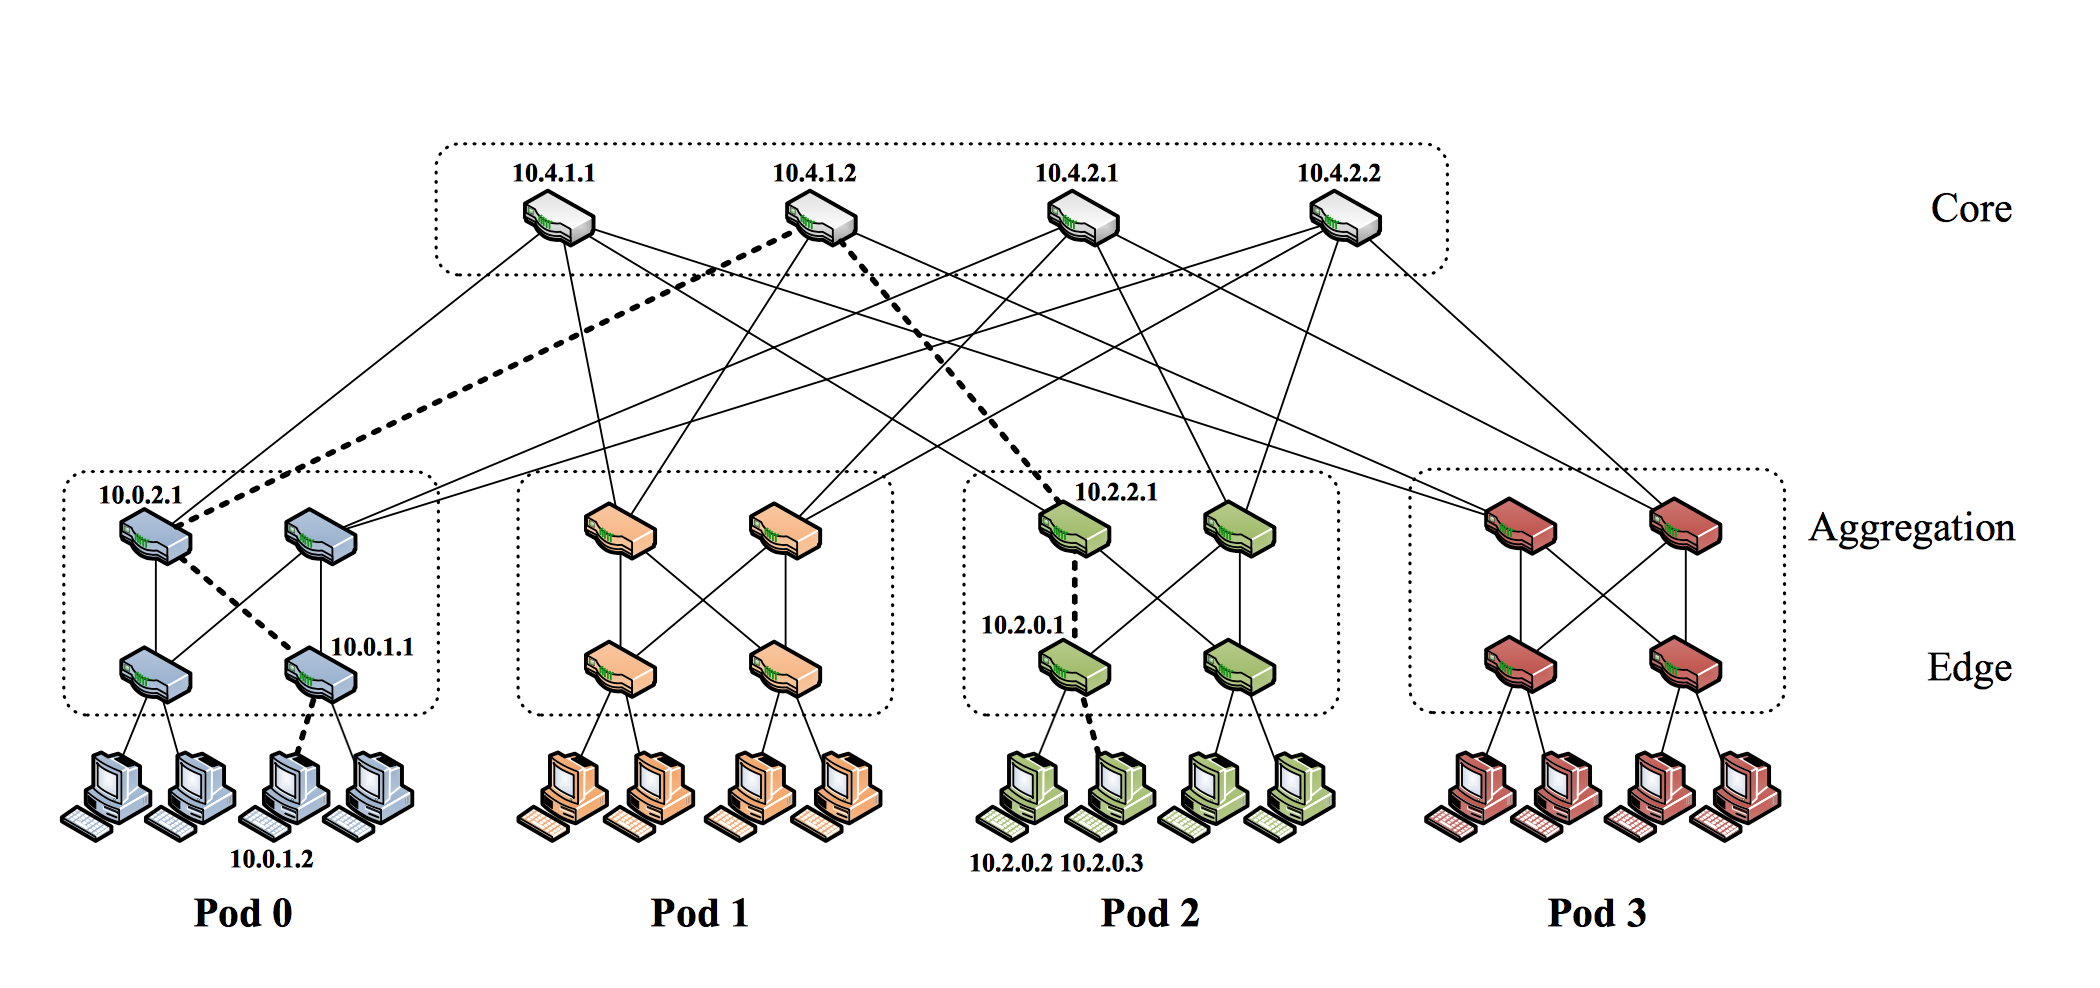
\includegraphics[width=0.9\columnwidth, right]{figures/fattree.png}
	\compactcaption{Fat Tree Topology with 3-level hierarchy.}
	\label{fig:fattree}
\end{figure}
Operators can leverage the network structure of topologies to reduce
the solution space by specifying undesirable path patterns.  For
example, the operator might require that a path between two edge switches in a
fat-tree does not traverse another edge switch.  This pattern doesn't
drastically reduce the set of possible paths due to the dense
interconnect between aggregate and core switches. 

We introduce \emph{tactics} (the name is inspired from the usage in SMT solvers, not 
proof assistants)
on labels; abstractions that allow a
network operator to impose restrictions on paths. 
We use the notion of mapping the set of switches to labels to 
have a coarse-grained way for specifying path patterns. Tactics on labels 
help create search strategies which can be used for groups
of packet classes instead of individual switch-level patterns which
lack generality.

 Let $Lb$ be the set of labels and $S$ be the set of switches in the topology. 
 Let $\phi : S \rightarrow Lb$ be the labeling function that maps each switch to a label in $Lb$. 
% One example for $\phi$ in the fat-tree topology in \Cref{fig:fattree} can be that we map all switches 
%therefore leveraging the hierarchical structure of the topology. 
For e.g., we can leverage the hierarchical structure of the fat-tree by
mapping all switches in the same level (core, aggregate or edge) to the same label.
A path $p$ is a word over the alphabet $S$. 
We define the path-labeling function $\Phi : S^* \rightarrow Lb^*$,  which maps each switch in the path to its corresponding 
 label. 
 For example, given the path $p = e1\ a2\ c3\ a4\ e2$, the path-labeling function function produces 
 $\Phi(p) = eacae$---maps each switch to its corresponding label.
 Here, $e$, $a$, and $c$ stand for edge, aggregate, and core respectively.

\subsection{Synthesis with Tactics}
%We use regular expressions and finite automaton to prune the constraints and impose restrictions on the path. The natural way for operators to specify tactics are using \emph{blacklists}, which specify what the path should not be. To express this in a intuitive manner, we use regular expressions on the set of labels to specify blacklists. For example, to blacklist paths from a edge switch to edge switch to not go through another edge switch, we can describe the tactic as $\neg (e .^* e .^* e)$ where the label of all edge switches is $e$. Another tactic is of the form $\neg (e (.)^4 a c .* e)$ which specifies we have a path of length 4, we do not go in the direction towards the core (as to reach the edge, the path would have to then go downwards from the core). 
Tactics are simple regular expressions over the set
 of labels and are used to blacklist certain path patterns.
Regular expressions have been previously used in tools like
NetGen~\cite{netgen} to specify the paths for a packet class.
While supporting full regular expressions is possible, it causes a blow-up in the solving time as further
constraints need to be added to the solver to ensure that a path satisfies the regular expression. 
Rather than specifying how the path must look like,
 we use regular expressions on switch labels to specify \emph{blacklists} i.e.,
what the path must \emph{not} look like. A tactic,
 for example, can blacklist paths from an edge switch to an edge switch that go through another edge switch. 
%\loris{we need a plot for the full regex thing to compare with Madhu, it would be great to repeat some of their experiments}

\subsubsection{Restricted Tactic Syntax} 
We specify tactics using a restricted set of regular expressions\footnote{
	It is a subset of star-free languages~\cite{starfree}.}
 that not only do not require extra constraints to be added,
but actually allow us to reduce the number of constraints in $\Psi$.
Tactics are regular expressions described by the following grammar:
$$\begin{array}{rcl}
R  &  :=  &  \neg (l_{src} .^i C .^* l_{dst}) \\
C  &  :=  &  \varepsilon \mid l_1 \mid l_1 l_2\\
\end{array}$$
where $l_i\in Lb$ and $l_{src}, l_{dst}$ are used to specify the labels of the source switch 
and destination switch, respectively.
Since our goal is to blacklist paths, we allow regular expressions to be negated at the outer level. 
\begin{example}
 $\neg (e .^i c .^* e)$ indicates that the path must not contain a core switch at the $(i+1)^{th}$ step. 
 Similarly, $\neg (e .^i .^* e)$ indicates that the path connecting two edge switches should have a length $ < i + 1$. 
\end{example}

Let $\pi = sw_0\ldots sw_k$ be a path for packet class $pc$
and let its labeling be $\Phi(\pi)= a_0\ldots a_k$.
We say that $\pi$ satisfies a tactic $R$,  $\Phi(\pi) \in L(R)$, if the following
holds:
\begin{compact2itemize}
\item $\Phi(\pi) \in L(\neg R)$ iff $\Phi(\pi) \not\in L(R)$;
\item $\Phi(\pi) \in L( l_{src} .^i .^* l_{dst})$ iff $k\geq i+1$, $l_{src}= a_0$, and $l_{dst}= a_k$; 
\item $\Phi(\pi)  \in L (l_{src} .^i l.^* l_{dst})$ iff $k\geq i+2$, $l_{src}= a_0$, $l_{dst}= a_k$, and $a_{i+1}=l$;
\item $\Phi(\pi)  \in L( l_{src} .^i l_1 l_2.^* l_{dst})$ iff $k\geq i+3$, $l_{src}= a_0$, $l_{dst}= a_k$, $a_{i+1}=l_1$, and $a_{i+2}=l_2$.
\end{compact2itemize}
In \Name, operators can specify conjunctions of tactics which adhere to the restricted 
syntax and the synthesis algorithm is modified to enforce the tactics. 
\begin{example}
The ``No Edge'' tactic ensures that a edge-edge path
cannot traverse another edge switch. It is expressed using conjunctions of tactics:
$\neg (e .^* e .^* e)\equiv \bigwedge \limits_{i=0}^{i=\mu-2} \neg (e .^i e .^* e)$ where $\mu$ is the limit on path length. 
The ``Valley-free'' Tactic:  $\neg (e .^5 .^* e)$ $\wedge \neg (e .^* e .^* e)$  
ensures that a edge-edge path is of the form $e-a-c-a-e$. 
\end{example}
Paths used in production datacenter networks adhere to both these
tactics~\cite{vl2-sigcomm09,jupiterrising-sigcomm15}. Such paths are
simple and make networks easy to manage and
troubleshoot~\cite{benson:complexity:nsdi2009}.

\subsubsection{Modified Synthesis Algorithm with Tactics}
In our synthesis algorithm, the reachability-propagation constraints (\Cref{eq:bckprop}) 
construct the path from destination to source. We use tactics to prune these constraints, so that
the path synthesized satisfies the tactic regular expression.  

The tactic set $\Gamma = \{(R_1, pc_1), \ldots, (R_n, pc_n)\}$
specifies that tactic $R_i$ is applied on packet class $pc_i$ where 
$pc_1, \ldots, pc_n$ $\in PC$ and $R_1,\ldots,R_n$ are regular
expressions satisfying the restricted tactic syntax. 
Given a tactic $R$ applied to a packet class $pc$, 
we define $\Psi_T(R,pc)$ as the additional SMT constraints used for 
synthesis such that  $(\Psi \wedge\ \bigwedge\limits_{(R, pc) \in \Gamma} \Psi_T(R,pc))$ 
is provided as input to the SMT solver.
	Note that $\Psi_T(R,pc)$ is presented as additional SMT 
constraints only for clarity. 
In practice, the modified synthesis algorithm will remove constraints for each 
$(R,pc)\in \Gamma$.
%In the first
%two cases, we remove some of the reachability constraints by adding negated unit clauses, 
%while we modify these constraints for the next two cases.
%To incorporate tactics in the path for packet class $pc$, we need to modify these constraints. For a path $\pi = sw_0 \ldots sw_k$ and labeling $\Phi(\pi) = a_0 \ldots a_k$, we describe the modifications of the constraints for each type of tactic.
%\loris{this part needs revision. Every time you say we remove constraints, but it actually looks like you are adding extra constraints
%of the form not(..)}

\noindent\textbf{Type 1.} For a tactic $R$ of the form $\neg (l_{src} .^i .^* l_{dst})$ applied to $pc$: 
\begin{equation} \label{eq:type1}
	\Psi_T(R, pc) = ~ \forall sw,k \geq i + 1. (sw,pc,k) \notin Reach
\end{equation}
This tactic restricts the path to a length $ < i + 1$. Thus, we can remove the reachability constraints  of \Cref{eq:bckprop} 
for all the tuples $(sw,pc,k) \notin Reach$ satisfying \Cref{eq:type1}
as they cannot contribute to any path satisfying the tactic.  

\noindent\textbf{Type 2.} For a tactic $R$  
of the form $\neg (l_{src}  .^i l .^* l_{dst})$ applied to $pc$:
\begin{multline} \label{eq:t1}
\Psi_T(R,pc) = \forall sw.~ \phi(sw) = l ~\wedge~ sw \not= dst \implies \\ 
(sw, pc, i + 1) \notin Reach
\end{multline}
The tactic ensures that a switch with label $l$ cannot be reached in $i+1$
steps, except if $l = l_{dst}$. In that case,
only the destination switch with label $l$ can be reached in $i+1$ steps as 
the path with labeling $l_{src}.^i l_{dst}$ satisfies the tactic. If $l \not= l_{dst}$, then
all switches with label $l$ cannot be reached in $i+1$ steps. For all tuples
$(sw, pc, i+1) \notin Reach$ satisfying \Cref{eq:t1}, we can remove the reachability constraints of \Cref{eq:bckprop}.


\noindent\textbf{Type 3.} For a tactic $R$  
of the form $\neg (l_{src}  .^i l_1 l_2 .^* l_{dst})$ applied to $pc$: 
\begin{multline} \label{eq:t3}
\Psi_T(R,pc) = \forall n_1, n_2.~\phi(n_1) = l_1~\wedge~ \phi(n_2) = l_2 ~\wedge~ n_2 \not=dst \\  \implies 
\neg (Reach(n_1, pc, i + 1) \wedge Fwd(n_1, n_2, pc))
\end{multline}
This tactic ensures that a switch with label $l_1$ at $i+1$ in the path
will not forward the packet to a switch with label $l_2$ (unless $n_2$ is the destination). 
To enforce this, we modify the \Cref{eq:bckprop} and remove all $l_1\rightarrow l_2$
edges at position $i+1$ in the path for which the switch with label $l_2$  is not the destination.  

%-> if a path is solution of modified constraint it satisfies regex
%<- if a path is solution of original constraints and satisfies regex, then it's a possible solution of modified constraints.

%Thm 6.1: Given a tactic R for the class pc, if \Pi |= \psi /\ Psi_R, then for every (\pi,pc)\in \Pi, \pi|=R (written a  bit better)
%
%Thm 6.2: Given a tactic R for the class pc, 
%if \Pi |= \psi, 
%and for every (\pi,pc)\in \Pi, \pi|=\psi_R,
%\Pi |= Psi_R.
We now state the soundness and completeness  
of the synthesis algorithm with tactics. 
Let $(Fwd, Reach)$ be a model of $\Psi$ and 
$\Pi = \texttt{paths}$ $(Fwd,$ $Reach)$ be the set
of induced paths (from Definition \ref{def:Pi}).
\begin{theorem}[Soundness]
	For a tactic set $\Gamma$, if $(Fwd, Reach) \models \Psi \wedge \bigwedge\limits_{(R, pc) \in \Gamma} \Psi_T(R,pc)) $, 
	then $\forall (R, pc) \in \Gamma. ~\forall(\pi', pc') \in \Pi. ~pc = pc' \implies \Phi(\pi') \in L(R)$.
\end{theorem}
\iffull
\begin{proof}
	\textbf{Assume} $\exists (R,pc) \in \Gamma$ such that $(\pi, pc) \in \Pi$ and $\Phi(\pi) \not\in L(R)$.
	Consider the three types of tactics for $R$: \newline
	\textbf{Type 1}: $R = \neg (l_{src} .^i .^* l_{dst})$ \\
	$\Phi(\pi) \not\in L(R)$ $\implies$ $\Phi(\pi) \in L(l_{src} .^i .^* l_{dst})$. \\
	Thus, $\pi = src\ sw_1 \ldots sw_i \ldots dst$. \\
	Therefore,  $(dst, pc, k_{dst}) \in Reach, k_{dst} \geq i + 1$. \\
	However, $(Fwd, Reach) \models \Psi_T(R, pc) \implies (Fwd, Reach) \models \forall sw,k \geq i + 1. (sw,pc,k) \notin Reach$.\\
	Contradiction, as $\exists sw, k \geq i + 1. (sw,pc,k) \in Reach$.
	\newline
	\newline
	\textbf{Type 2}: $R = \neg (l_{src} .^i \ l \ .^* l_{dst})$ \newline
	$\Phi(\pi) \not\in L(R)$ $\implies$ $\Phi(\pi) \in L (l_{src} .^i \ l \ .^* l_{dst})$. \\
	Thus, $\pi = src\ sw_1 \ldots sw_i \ sw_{i+1} \ldots dst$ such that $\phi(sw_{i+1}) = l$. Also $sw_{i+1} \not=dst$ (dst has to be the last switch in $\pi$)\\
	Therefore,  $(sw_{i+1}, pc, i+1) \in Reach$. \\
	However,
	$(Fwd, Reach) \models \Psi_T(R, pc) \implies (Fwd, Reach) \models \forall sw.~ \phi(sw) = l ~\wedge~ sw \not= dst \implies  (sw, pc, i + 1) \notin Reach$. \\
	Contradiction, as $\exists sw. ~ \phi(sw) = l ~\wedge~ sw \not= dst \wedge (sw,pc,i+1) \in Reach$.
	\newline \newline
	\textbf{Type 3}: $R = \neg (l_{src} .^i \ l_1 \ l_2 \ .^* l_{dst})$ \newline
	$\Phi(\pi) \not\in L(R)$ $\implies$ $\Phi(\pi) \in L (l_{src} .^i \ l_1 \ l_2 \ .^* l_{dst})$. \\
	Thus, $\pi = src\ sw_1 \ldots sw_i \ sw_{i+1} \ sw_{i+2} \ldots dst$ such that \newline $\phi(sw_{i+1}) = l_1, \phi(sw_{i+2}) = l_2$. Also $sw_{i+2} \not=dst$ (dst has to be the last switch in $\pi$)\\
	Therefore,  $(sw_{i+1}, pc, i+1) \in Reach \wedge (sw_{i+1}, sw_{i+2}, pc) \in Fwd$. \\
	However,
	$(Fwd, Reach) \models \Psi_T(R, pc) \implies (Fwd, Reach) \models \forall n_1, n_2.~\phi(n_1) = l_1~\wedge~ \phi(n_2) = l_2 ~\wedge~ n_2 \not=dst  \implies 
	\neg (Reach(n_1, pc, i + 1) \wedge Fwd(n_1, n_2, pc))$. \\
	Contradiction, as $\exists n_1. n_2. ~\phi(n_1) = l_1~\wedge~ \phi(n_2) = l_2 ~\wedge~ n_2 \not=dst \wedge Reach(n_1, pc, i + 1) \wedge Fwd(n_1, n_2, pc)$. 
\end{proof}
\fi

\begin{theorem}[Completeness]
For a tactic set $\Gamma$, if $~\Pi \models \Psi$ and 
$\forall (R, pc) \in \Gamma. ~\forall(\pi', pc') \in \Pi. ~pc = pc' \implies \Phi(\pi') \in L(R)$
then $\forall (R, pc) \in \Gamma. (Fwd, Reach) \models \Psi_T(R, pc)$.
\end{theorem}
\iffull
\begin{proof}
	\textbf{Assume} $\exists (R, pc) \in \Gamma$ such that $(\pi, pc) \in \Pi$ and \newline 
	$(Fwd, Reach) \not\models \Psi_T(R,pc)$.
	Consider the three types of tactics for $R$: \newline
	\textbf{Type 1}: $R = \neg (l_{src} .^i .^* l_{dst})$ \newline
	$(Fwd, Reach) \not\models \Psi_T(R, pc) \implies (Fwd, Reach) \not\models \forall sw,k \geq i + 1. (sw,pc,k) \notin Reach$ \newline
	Therefore $\exists sw, k \geq i + 1. (sw,pc,k) \in Reach$. \\
	Therefore, $\Phi(\pi) \in L(l_{src}\ .^i \ .^* \ \phi(sw) \ .^* \ l_{dst}) \implies \Phi(\pi) \in L(l_{src} .^i .^* l_{dst}).$\\
	Contradiction, as $\Phi(\pi) \in L(R)$.
	\newline 
	\newline 
	\textbf{Type 2}: $R = \neg (l_{src} .^i \ l \ .^* l_{dst})$ \newline
	$(Fwd, Reach) \not\models \Psi_T(R, pc)$ $\implies$ $(Fwd, Reach) \not\models$ \newline $\forall sw.~ \phi(sw) = l ~\wedge~ sw \not= dst \implies  (sw, pc, i + 1) \notin Reach$. \\
	Therefore $\exists sw. \ sw \not= dst \ \wedge \ \phi(sw) = l \ \wedge \ (sw,pc,i+1) \in Reach$. \\
	Therefore, $\Phi(\pi) \in L( l_{src}\ .^i \ l \ .^* \ l_{dst})$. \\
	Contradiction, as $\Phi(\pi) \in L(R)$. 
	\newline  
	\newline
	\textbf{Type 3}: $R = \neg (l_{src} .^i \ l_1 \ l_2 \ .^* l_{dst})$ \newline
	$(Fwd, Reach) \not\models \Psi_T(R, pc)$ $\implies$ $(Fwd, Reach) \not\models$  \newline
	$\forall n_1, n_2.~\phi(n_1) = l_1~\wedge~ \phi(n_2) = l_2 ~\wedge~ n_2 \not=dst  \implies 
	\neg (Reach(n_1, pc, i + 1) \wedge Fwd(n_1, n_2, pc))$. \\
	Therefore $\exists n_1, n_2. ~\phi(n_1) = l_1~\wedge~ \phi(n_2) = l_2 ~\wedge~ n_2 \not=dst ~\wedge~ Reach(n_1, pc, i + 1) ~\wedge~ Fwd(n_1, n_2, pc)$. \\
	Therefore, $\Phi(\pi) \in L(l_{src}\ .^i \ l_1~l_2 \ .^* \ l_{dst})$. \\
	Contradiction, as $\Phi(\pi) \in L(R)$.
\end{proof}
\fi

The intuition behind the restricted tactic syntax comes from the structure of the reachability propagation 
constraints (\Cref{eq:bckprop}) which construct the path for a packet class. 
Each constraint enforces that if a switch is reachable in $k$ steps in a path,
 there must a neighbour switch in the path reachable at $k-1$ steps. 
Using the $Reach$ relations, we can specify path length restrictions (Type 1)
 or prevent switches with a certain label at some position (Type 2). 
 The structure of \Cref{eq:bckprop} restricts regular expressions on only local switch
 neighbours (Type 3).
  The structure of these constraints 
  prevents us from being able to specify unrestricted regular expressions (supporting
  these would require adding additional constraints).
  \begin{example}
  Consider a tactic $\neg(e .^i a c a .*e)$. To enforce
  this tactic, we need to have constraints which prevent the path reaching an aggregate switch in $i+3$
  steps when the path traverses an aggregate and core switch at $i+1$ and $i+2$ steps
  respectively. This cannot be specified by modifying the reachability 
  constraints in its current form, 
  because the constraints for reachability for a switch in $i + 3$ steps only depends on 
  the constraints for reachability in $i+2$ steps. 
   \end{example}

Tactics are heuristics, but well-defined ones with formal semantics and provable soundness properties.
 In practice, tactics can be used to specify restrictions which would not reduce the search space dramatically, 
but are still useful toward speeding up the synthesis, especially in datacenter topologies which are hierarchical 
 and can be used to specify interesting tactics. One of the biggest advantages
 of tactics is that it is \emph{policy-agnostic} since it enforces conditions on the path, and
 can be used in conjunction with the different policies supported by \name (isolation, traffic engineering etc.).  
 Thus, we have provided a framework for the
 development of search strategies based on path properties, and 
operators can design tactics based on the physical topologies (datacenter topologies are hierarchical)
 to create a library of tactics that can be reused for workloads.
  While tactics sacrifice completeness, operators can discard the tactic 
  if synthesis fails and use \name without tactics.
%\loris{For that restricted set of regexes the algorithm is trivial you should write the first pass. 
%See the simplified syntax.
%I'll help you with the proof but essentially you have to show that
%if a path $sw_1\ldots sw_k$ satisfies the tactic regex then it is removed (i.e. all constraints necessary
%for it to be encoded have been removed).
%Other direction: if a path was in the original set of constraints and did not 
%satisfy the tactic it has not been removed (also pretty easy)
%}
%\kausik{I think the tactics are quite intuitive to not need a proof of correctness. Do you think we need to explain how we came upon the restricted syntax?
%}
%\loris{No proof is fine. Some intuition would help. Give an example of one that locality can't handle.}

%\subsection{Label Pruning}
%Tactics are an intuitive way to express path properties leveraging the network structure using regular expressions. However, not every permutation of the label alphabet is a valid path in the topology, for example $eaae$ as the aggregate switches are only connected to edge or core switches. Under closer inspection, for a path from an edge switch to another edge switch, we can see that aggregate switches can only occur at odd path length. We describe a label automaton and the algorithm to prune constraints using switch label adjacencies. 
%
%To pruning the constraints using network labels, we construct a label automaton for the topology. The label automaton $A^L$ is an automaton which accepts all words over the alphabet $Lb$ which are a labeling of a valid path in the topology in the topology and rejects all other words. The label automaton has state for each label and transitions for those labels which are connected to that label. We construct the label automaton for the fat-tree topology(\cref{fig:fattree}) in \cref{fig:labelauto}.  
%
%\begin{figure}[h!]
%	\centering
%	\begin{tikzpicture}[shorten >=1pt,node distance=2cm,on grid,auto] 
%	\node[state,initial] (q_0)   {$q_0$}; 
%	\node[state,accepting] (q_a) [right=of q_0] {$q_a$}; 
%	\node[state, accepting] (q_e) [above=of q_a] {$q_e$};
%	\node[state,accepting] (q_c) [below=of q_a] {$q_c$}; 
%	\path[->] 
%	(q_0) edge  node {e} (q_e)
%	edge node {a} (q_a)
%	edge node {c} (q_c)
%	(q_e) edge [bend right=30]  node {a} (q_a)
%	(q_a) edge [bend right=30] node {e} (q_e)
%	edge [bend right=30] node {c} (q_c)
%	(q_c)[bend right=30] edge node {a} (q_a);
%	\end{tikzpicture}
%	\caption{Label automaton $A^L$ for fat-tree topology}
%	\label{fig:labelauto}
%\end{figure}
%For a path starting from an edge switch,  
%using a dynamic programming approach, we build sets $\Gamma(k)$ which is the set of all words starting with $e$ and of length $k$ accepted by the label automaton $A^L$ : $w \in \Gamma(k) \Leftrightarrow w \in L(A^L) \wedge |w| = k$. The algorithm computes $\Gamma(k-1)$, and then the last character of each word can be used to find the state the automaton is in(the automaton reaches the state after reading a particular label), and make a valid transition from that state to construct a word of size $k$ to compute  $\Gamma(k)$. 
%
%Let us define $\Delta(k) := Lb \setminus \{l \ | w \in \Gamma(k) \wedge w[k] = l\}$ to the set of labels which cannot be reached by a path of length $k - 1$ (the length of the label word is one more than length of the path) from an edge switch. For example, in the fat-tree topology in \cref{fig:fattree}:
%\[
%\Delta(1) = \{c, e\} \ \ \ \Delta(2) = \{a\} \ \ \ \Delta(3) = \{c,e\}
%\]
%For each $k \leq \mu$, we can add the following constraints for packet classes which have traverse from a edge-to-edge switch to prune the backward reachability propagation constraints \cref{eq:bckprop}: 
%\begin{equation}
%	\forall sw. \phi(sw) \in \Delta(k) \implies (sw, pc, k -1) \notin Reach
%\end{equation}
%The label automaton pruning is sound and complete because we are using the network structure and network labels to prune certain constraints which cannot be valid, without imposing any restrictions on the path. 

%\section{Network Surgery}
%Network surgery is the technique of performing equivalent network transformations to eliminate redudant constraints required for synthesis of switch rules. One of the properties of the path found by the synthesis solver is that it is simple (i.e no loops). Using this property, we can create slices of the topology where a packet class' path will reside completely, thus not requiring to add constraints for switches in other slices of the topology. 
%
%To create the topology slices, we use Schmidt's linear-time algorithm\cite{schmidt} to find bridges in the graph. A bridge is an edge in the topology, which when removed, partitions the graph into two disconnected components. <write-about-slices>. 
%
%Consider a reachability policy where the source and destination switches belong to the same topology slice. Since, the bridge edge is the only edge connected vertices of this slice with the rest of the graph, the path for the reachability policy will be contained in the topology slice and not cross the bridge (otherwise the path would have to traverse through the bridge twice back and forth which is not permitted). 
%
%Formally, let us define the slices of the topology as $S_1$, $S_2, \ldots S_n \subset S$. We define the slice neighbour function for the slices as $N_{S_i}(s) = \{v | v \in S_i \wedge (s,v) \in L\}$. If there is a reachability policy $(r, pc)$ with $src,dst \in S_i$, we can replace the switch domain $S$ by $S_i$ and the neighbour function $N$ by $N_{S_i}$ in the constraint formation for reachability. For example, the backward reachability propagation constraints for a policy in slice $S_i$ can be modified to : 
%\begin{multline}
%\forall n_1,k.  n_1 \in S_i \wedge Reach(n_1,pc,k) \implies \exists n_2. n_2 \in N_{S_i}(n_1) \\ \wedge  Reach(n_2,pc,k-1) \wedge Fwd(n_2,n_1,pc)
%\end{multline}
%For packet classes isolated with packet class $pc$, only links in $S_i$ are needed to be isolated, as the path will be confined to topology slice $S_i$. 


\section{Divide-and-Conquer Synthesis} \label{sec:optimistic}
%\aditya{I haven't read earlier tech sections yet. we need to make sure ``packet class'' is defined somewhere, as it is an unusual term. also, we need to figure out how we are using ``policy''.}

One of the key challenges to the synthesis performance is the number
of packet classes synthesized and the policy interactions among them
(isolation, capacity, etc.). Since the complexity of finding a
forwarding plane configuration is roughly \emph{exponential} in the
number of packet classes, the synthesis time shoots up with increasing
packet classes. 
We notice that since datacenter topologies have a dense interconnection of
links between layers there can be
numerous different forwarding plane configurations as solutions.
% \aditya{previous sentence does not parse} 
We propose a heuristic approach which partitions the problem 
into smaller components to speed up synthesis.

The intuition is as follows, suppose we have two packet classes $pc_1,
pc_2$ isolated from one another, the standard synthesis algorithm adds 
constraints for both packet classes to the solver for finding the solution.
Instead, we could synthesize $pc_1$
independently and, after that, find a solution for $pc_2$ 
that is isolated from the
path obtained for $pc_1$. We term this
procedure \emph{divide-and-conquer} synthesis, as we divide
the problem and try to synthesize them separately.
However, synthesis of $pc_2$ can fail because the solution
of $pc_1$ may be such that there is no way to place an isolated path for
$pc_2$ but if they have been synthesized together, a
solution might exist. To improve effectiveness, we integrate the 
divide-and-conquer approach with recovery 
mechanisms discussed in \Cref{sec:recovery}.

\begin{algorithm}[h]
\begin{footnotesize}
	\floatname{algorithm}{Pseudocode}
	\caption{Divide-and-Conquer Synthesis}
	\label{dcsyn}
	\begin{algorithmic}[1]
		\Procedure{DCSyn(P)}{}
		\If{$size(P) < P_{thres}$}
		\State{Apply normal synthesis on P}  
		\Else
		\State{Partition P into $P_1$ and $P_2$}
		\If{interpartition edges $> E_{thres}$} \State{Apply normal synthesis on P} \EndIf
		\State{F = []  \hspace{1cm} /* Failed solutions */}
		\State{attempts = 0} 
		\While{$attempts < RA_{max}$}
		\State{$sol_1$ = Apply  synthesis on $P_1$ such that $sol_1 \notin F$}
		\If{synthesis($P_1$) fails} \State{\Return DCSyn failure} \EndIf
		\State{$sol_2$ = Apply synthesis on $P_2$ such that \newline \hspace*{2cm} $sol_2 + sol_1$ is a solution for P}
		\If{synthesis($P_2$) fails} 
		\State{F.append(unsat-cores($P_2$))}
		\State{attempts++}
		\Else
		\State{\Return DCSyn success}
		\EndIf
		\EndWhile
		\State{\Return DCSyn failure}
		\EndIf
		\EndProcedure
	\end{algorithmic}
\end{footnotesize}
\end{algorithm}



%% $pc_1$ would have been different.

We define a policy graph $P = (R, I)$ where every vertex $r \in R$
is a packet class for a reachability/waypoint policy and edges
denote isolation constraints between packet classes.
%\aditya{again the
%  use of packet class and policy here is unconventional and needs to
%  be carefully defined early on} 
An edge $(r_1,r_2) \in I$  means that the paths of $r1$ and $r2$ are
isolated from each other. We assume that there are no capacity policies
in the input specifications. 
%since isolation is a local policy 
%in the sense that correct enforcement of isolation only requires information of neighbours
%\loris{don't know what this last sentence means}. 
%Resource managements policies like link capacity policies are global,
% and thus difficult to reason about them in smaller components.
  Given the policy graph $P$, we
can synthesize each connected component independently, since packet
classes in different connected components are not related by any
isolation policy, and therefore are independent of each other.

We describe the heuristic synthesis procedure in Pseudocode 1,
which takes as input a connected component of the policy graph.
 The crux of the procedure is that we partition each connected component $P$
  into two smaller components $P_1$ and $P_2$
  and do the following:
%   \aditya{are these
%  two connected components? if so, there will be no policy interaction
%  across them, no? given that, the following statement seems
%  incorrect} 
1) synthesize $P_1$ and obtain a solution $S_1$, and
2) for packet classes of $P_2$ that are
isolated to packet classes in $P_1$, 
%\aditya{this seems incorrect: no such packet classes exist?} 
add the solution $S_1$ as a constraint to ensure that the
packet classes in $P_2$ will not share the edges of the respective
paths obtained in $P_1$. 
%The difference from
%normal synthesis for a isolation policy is that since we don't have
%the paths for both packet classes, we add isolation constraints at all
%switches (\cref{eq:isolation})
%\loris{don't know what previous and next sentence means. Please rewrite clearly}. 
%In contrast, if we had a solution for
%one packet class, we need to ensure the other path is isolated only at
%the switches visited by the path of the solved packet
%class. 
%\aditya{it seems from the rest of the description below that p1
%  and p2 are not two connected components; they are just subgraphs. if
%  so, the ending sentence of the previous paragraph that talks about
%  connected components is misleading because that is not actually what
%  we do}
%\aditya{I did not look at the pseducode}

We use two schemes to partition the policy graph connected component into two: the
first one is \emph{min-cut} partitioning, which partitions the graph
such that inter-partition edge count is minimized. The
rationale behind the heuristic is that since we intend to perform the
synthesis of both partitions separately, the partition should maximize
the isolation policies within components and minimize across
components. By maximizing isolation policies during synthesis of the
component, the partial solution is more likely to be compatible with a
complete solution. However, if the min-cut partitioning produces a
component smaller than a threshold size, we perform partitioning of
the graph into two equal sized partitions and minimizing the cut edges
between the partitions. We need to ensure that we don't partition the
graph smaller than a threshold, as the partial solutions obtained by
synthesis of very small partitions are more likely to conflict with
other packet classes. Our implementation of \Name performs
divide-and-conquer synthesis recursively on the components till we cannot partition the
component further. 

\subsection{Solution Recovery} \label{sec:recovery}
While in the best case divide-and-conquer synthesis  will lead to a great
increase in performance, we need a recovery mechanism in case we cannot find
compatible partial solutions.  We describe a bounded \emph{solution} recovery
scheme in \Cref{dcsyn} \kausik{Add refs here}integrated with the divide-and-conquer
synthesis procedure.  Many SMT solvers track constraints and return
an unsatisfiable core~\cite{unsatcores} when synthesis fails. Informally,
the unsatisfiable
core is a set of tracked constraints\footnote{
	Not necessarily a minimal set of constraints.}
 that describe why there wasn't a feasible 
solution. This helps us track failed partial solutions. 
%  in the synthesis of $P_2$
%by tracking the constraints added to ensure isolation with the paths
%of $P_1$.  
Thus, if synthesis of $P_2$ fails, the unsatisfiable cores
obtained from Z3 will be the paths of the solution of $P_1$ which are
causing the synthesis of $P_2$ to fail. 
When performing synthesis of $P_1$
again, we therefore ensure that we get \emph{different} paths from the
unsatisfiable cores we extracted.  Basically, we perform a 
\emph{solver-guided} enumeration of different solutions of $P_1$ to
find a satisfying solution for $P_2$ for faster convergence.

There are drawbacks to performing recovery. Since, recovery is a 
form of enumeration, in cases where the graph is highly constrained
(clique), finding a solution can lead to increased number of enumerations,
while synthesis without partitioning would provide a solution faster. 
Thus, we bound the number of enumerations performed by the 
recovery mechanism and return failure to find a solution by solution recovery
if we don't obtain a solution. 

Divide-and-conquer synthesis with recovery is sound, but 
it is incomplete as we bound the
number of enumerations. The success of this approach
is directly related to the size of the components (determined by $P_{thres}$). 
This is because, by synthesizing more packet classes together, we decrease the
conflicts arising between partial solutions. The extreme case is when we do not 
partition the component at all (normal synthesis), which is complete. 
Thus, to make the synthesis complete with faster convergence, we
perform iterations of divide-and-conquer synthesis, and at each iteration we double the
partition threshold $P_{thres}$ if the previous iteration failed. 
% \aditya{when is this doubling done? during one of the
%	recursive invocations, or only at the beginning?} 
This scheme tries to balance the trade-off between completeness, which
requires larger components, and performance, as synthesis is faster on smaller
components. 
In the extreme case, after $O(log~P)$
iterations, $P_{thres} > P$ and the divide-and-conquer synthesis routine cannot partition the graph any further,
thus rendering the routine complete. 
% \aditya{I
%	don't see this. you may not find a solution, no?}. In the extreme
%case, $P_{thres} \geq P$ and the algorithm will perform normal
%synthesis, and thus become complete. In a case when this happens
%\aditya{this is vague. what does ``this'' mean? are you saying
%	whenever doubling happens perf is degraded? if so, why do it?}, the
%performance of optimistic synthesis is degraded.
%However, synthesizing $P$ completely
%without partitioning would be faster than performing optimistic
%synthesis (densely connected like a clique) and enumerating as it
%would fail more often \aditya{this sentence is wierd. are you trying
%  to say that synthesizing P is faster in *some* cases?}. Thus, we
%bound the number of recovery attempts to ensure that we can say that
%optimistic synthesis has failed and perform normal
%synthesis. \aditya{need to be precise. what does ``to ensure that we
%  can say...'' mean}
 
 This synthesis approach is more \emph{effective}
 when there is a large number of solutions and provides a
 significant improvement. When the problem is highly 
 constrained and the number of solutions is low, 
 the recovery mechanisms and multiple iterations could 
 lead to a degraded performance. 
% by the optimistic synthesis 
% routine. 
 We evaluate the performance improvement of divide-and-conquer
 synthesis with varying isolation workloads in \Cref{sec:optimisticeval}.
 One of the major drawbacks of the divide-and-conquer approach is that it is very
 difficult to apply to global policies (like traffic engineering) primarily because
 splitting the input problem isn't easy, and development
 of strategies to speed-up global policies is a direction of future work.

 %\aditya{the last para was very vague. rest of the section was OK, modulo my comments}
 
%

\begin{figure*}
	\centering
	\subfloat[Baseline]{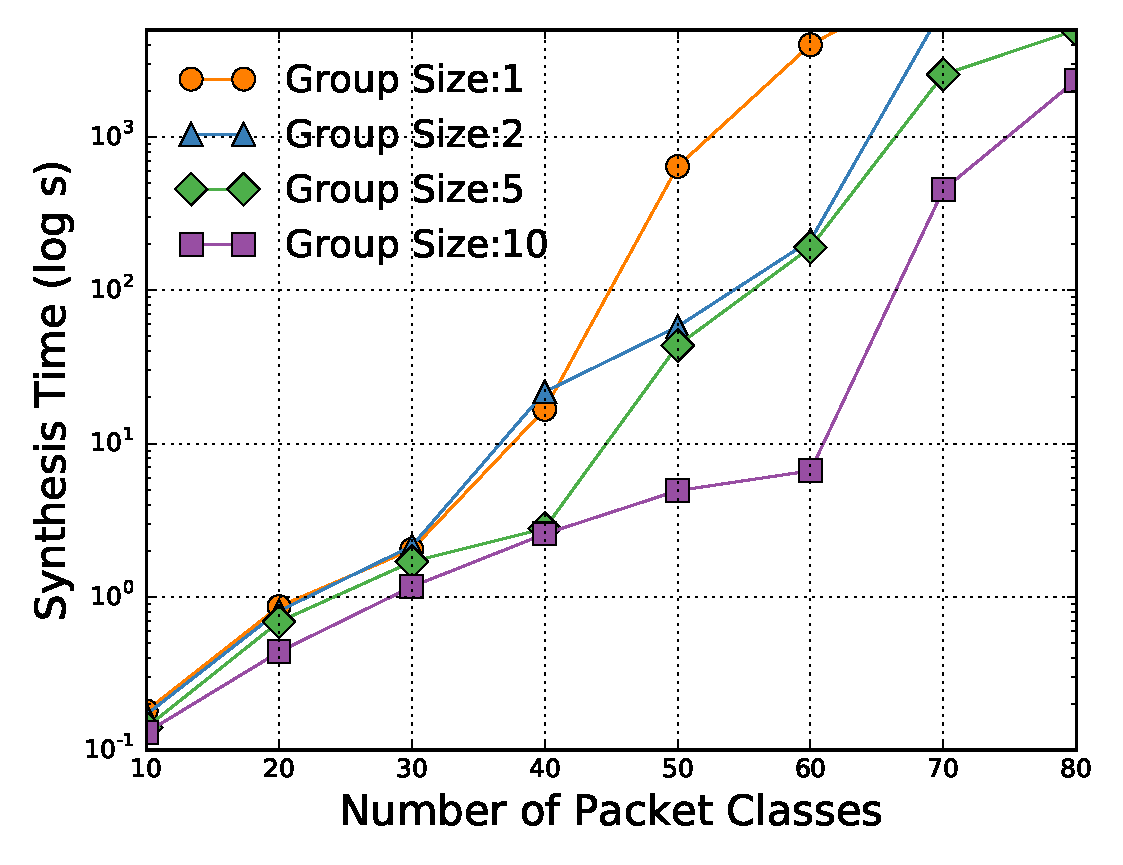
\includegraphics[width=0.66\columnwidth]{figures/noTacticIsolation.eps}}
	\subfloat[No Edge Tactic]{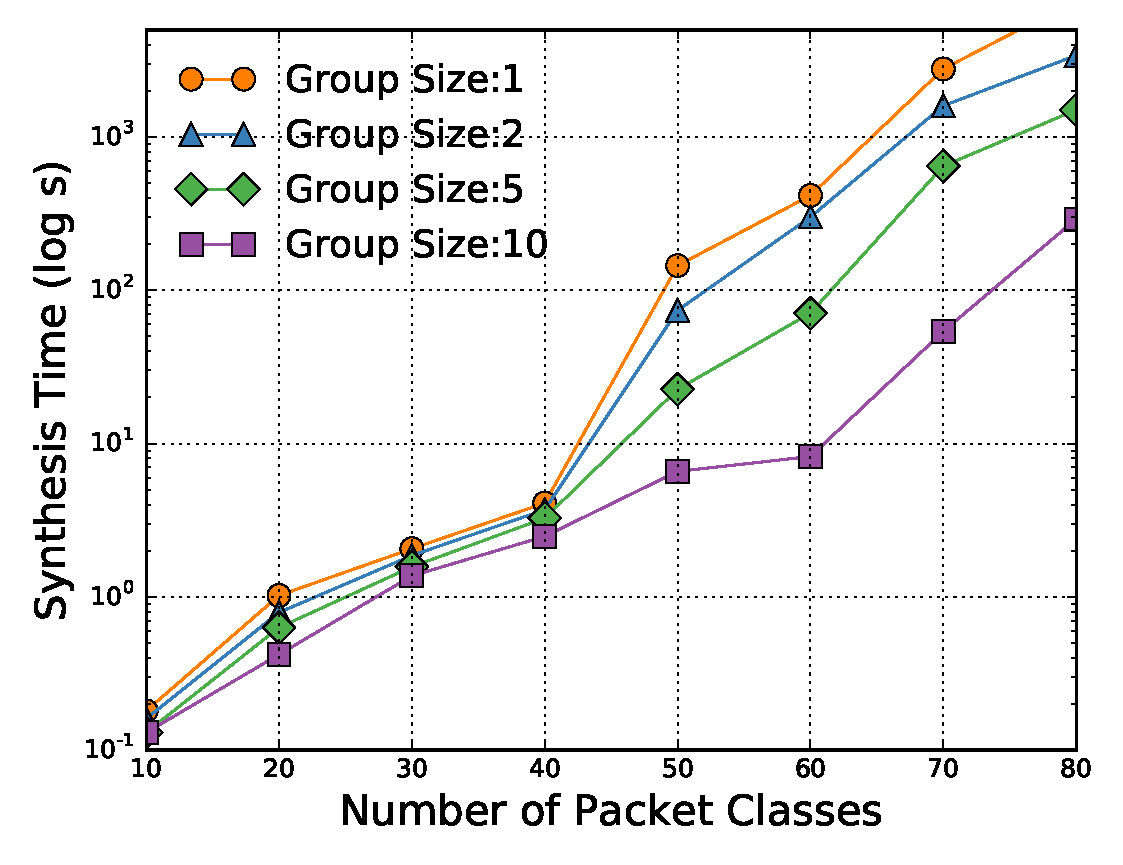
\includegraphics[width=0.66\columnwidth]{figures/edgeTacticIsolation.eps}}
	\subfloat[Valley-free Routing Tactic]{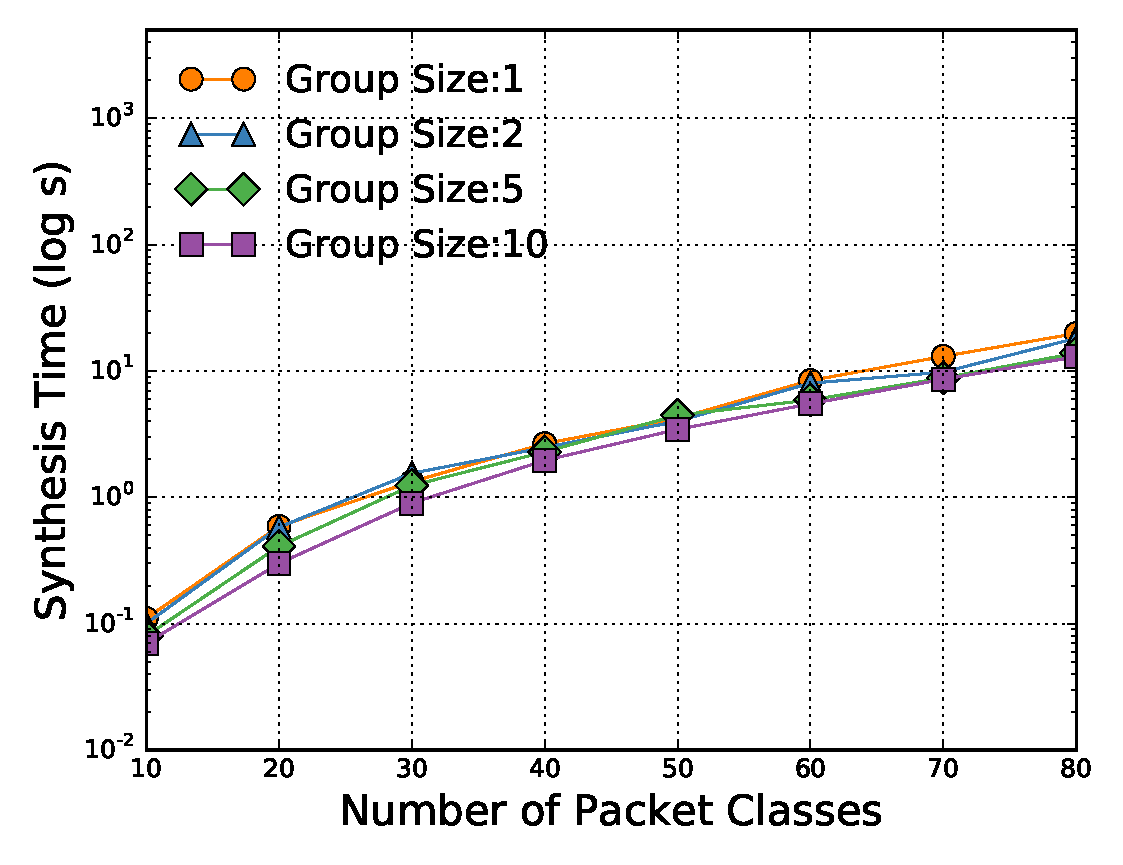
\includegraphics[width=0.66\columnwidth]{figures/noValleyTacticIsolation.eps}}
	\compactcaption{\label{fig:isolation}
		Total synthesis time (log scale) for isolation workloads over range of packet classes and different tenant-group sizes.}
\end{figure*}

\section{Evaluation} \label{sec:evaluation}

We implemented a full working
prototype of \Name in Python. We have implemented an interpreter for
the Genesis Programming Language using PLY~\cite{ply} and the synthesizer using 
the SMT solver Z3~\cite{z3} and its $\nu Z$ extension for MaxSMT and linear
 optimization~\cite{nuz3}; \name outputs the
forwarding rules for the switches, which can be provided as input to a
SDN controller (e.g., Floodlight~\cite{floodlight}) to install over the
network. \Name uses the Metis graph-partitioning library~\cite{metis}
to perform equi-sized partitioning 
used by divide-and-conquer synthesis. 
%We plan to make the code for \Name publicly available.

In this section, we evaluate \Name using
%\loris{really don't like the word realistic}
enterprise-scale multi-tenant data
center settings. 
Specifically, we ask:
\begin{compactitemize}
\item What is the performance of \Name's baseline synthesis
  algorithm for tenant policies? How does the performance vary with size of the
  network, number and the nature of policies in use? (\secref{sec:baselineeval})
  
  \item What is the performance of \name for operator policies
  like capacity bounds, traffic engineering, and network repair
  which use SMT with linear optimization objectives and MaxSMT? (\secref{sec:optimizationeval})

\item How much do tactics help improve \Name's 
  performance? Which tactics offer the best improvement? (\secref{sec:tacticeval})

\item To what extent does the divide-and-conquer synthesis improve \Name's
  performance? When does it lead to degraded synthesis times? (\secref{sec:optimisticeval})

\end{compactitemize}
%\loris{if you say this here don't write it in the bullet points}
Our experiment settings have a few thousand servers, tens of switches,
and hierarchical fat-tree network topologies which reflect a private
datacenter. Our experiments are parameterized by: (a) total size of
the fat-tree network (45-180 switches), (b) number of
tenants (1-80), and (c) number of packet classes in a tenant (1-10).
Note that a single packet class can be used to specify policy
for multiple host-pairs of a tenant connected to the 
same edge switches, and placement of the hosts can take uniformity
of policy in account to reduce the explosion of packet classes with 
increasing hosts.

Our primary metric of interest is synthesis time, measured in
seconds. In measuring this, we focus on the time the Z3 solver takes
to solve the constraints\footnote{
	We do not account for
constraint generation time in our evaluation, as it 
has polynomial time complexity and thus, can scale well unlike
constraint solving time;
a well-engineered system can considerably reduce
the constraint generation overheads.}. 
All experiments were conducted using a
32-core Intel-Xeon 2.40GHz CPU machine and
128GB of RAM. For evaluating the baseline performance, we impose a
synthetic limit on the path length $\mu$ to be $10$, which is adequate 
for a fat-tree topology with three levels. 

\subsection{Baseline Synthesis Performance for Tenant Policies} \label{sec:baselineeval} 
\minisection{Multi-Tenant Isolation} To evaluate the baseline
performance of \Name, we model a multi-tenant 80 switch
 topology with tenant-isolation in
\Cref{fig:isolation}(a).  For each workload we have $n$ tenants with
group size $g$ which is the number of packet classes for each
tenant. The x-axis shows the total packet classes $n*g$.  Packet
classes of a tenant are not isolated (and they implement simple
reachability within the tenant), while packet classes of different
tenants are traffic-isolated. Thus, no two tenants share a link in
the same direction, and can never
affect each other's performance.  We randomly\footnote{ Smarter
  placement of tenants could speed-up synthesis as tenant endpoints
  would be located closer to each other. The placement algorithm can
  be used to develop specialized tactics.}  place endpoints for the
tenants' packet classes, ensuring that no more than 4 tenants share a
single edge switch.  Operators can aggregate a tenant's traffic from
multiple instances connected to the same switches 
as a single reachability policy and establish
pathways for communication amongst different switches.

For a fixed group size, we observe that the total synthesis time
increases exponentially with number of packet classes.  As
 group size decreases, for the same number of classes, the 
number of tenants increases, increasing the number of isolation policies
and the synthesis times. 
Group size 1 denotes the
extreme case where all flows are isolated with each other.
 
While we evaluated a multi-tenant isolation setting, there are other
scenarios that translate to these workloads. Consider an example where
specific flows of tenants require QoS guarantees and these flows must
be isolated w.r.t. all other flows. This translates to a two-tenant
isolation setting. Operators can provide weaker isolation such that
two flows must be isolated on only certain ``special" links. 
This is an easier problem to tackle than isolation over all
links, and the performance of such scenarios would be better. 
Failure resiliency uses link-isolation policies which exhibit a similar
performance compared to the workloads considered here. 

\minisection{Effect of Topology Size} To evaluate \Name across
increasing topology sizes for isolation workloads, we fix the
tenant-group size to 5, and for each topology, we maintain the ratio
of packet classes to number of edge-aggregate links to 0.25.  We
choose this metric because if we keep the number of classes constant,
as topology sizes increases, it is easier to find isolated
paths due to more links. Thus, by keeping the number of packet classes proportional to
size of the topology, we maintain the relative difficulty of the
workload across topologies.  We show the average synthesis time per
class with increasing topology sizes in
\Cref{fig:tactic-topo} (baseline trace).  We are able to synthesize forwarding rules
for 12 tenants with group size 5 in a 125 switch topology in 124
seconds (avg. 2 seconds per traffic class).
 %Some comment I dont understand.
We also observe that average time per flow increases exponentially
with larger topologies, thus synthesis times are also exponential
\begin{wraptable}{l}{8em}
	\begin{footnotesize}
		\begin{center}
			\begin{tabular}{P{3em}| P{4em}}
				Number of Waypoints & Avg. Synthesis time per Class (s) \\
				\hline
				1 & 0.034\\
				
				2 & 0.138\\ 
				
				3 & 0.983\\ 
				
				4 & 15.41\\ 
				
				5 & 32.93\\
			\end{tabular}
		\end{center}
		\compactcaption{Average synthesis time per class for waypoint policies with increasing number of waypoints. } \label{tab:waypointeval} 
	\end{footnotesize}
\end{wraptable} 
in the number of switches.

\minisection{Waypoint Policies} To evaluate \Name's performance for
ordered sets of waypoints, we fix the number of waypoints (range:1-5)
 and generate 100 waypoint policies with different sizes and permutations
 of the ordered waypoint sets for a 80 switch topology.
 Each policy has edge switches as endpoints and randomly picked core or
aggregate switches for waypoints. The synthetic limit $\mu$ on the
path length is increased to 15 and no tactics are used 
(difficult to devise a tactic for the path satisfying a waypoint policy). The
average synthesis time for a waypoint policy is reported in
\Cref{tab:waypointeval}.  We observe that synthesis time increases
exponentially with total number of waypoints in a packet class's
policy, owing to the complexity of the problem.  \Name can synthesize
rules for a path with 3 total waypoints in less than a second, on
average. 
%\aditya{I don't follow this last sentence}


\subsection{Baseline Synthesis Performance for Operator Policies} \label{sec:optimizationeval}
\minisection{Isolation with Link Capacity Policies}
\Cref{fig:link-capacity} (baseline trace) 
shows the average synthesis time per flow for the same setting as above, but
additionally, there are 10 low-bandwidth links in the network for which the operator
specifies capacity policies (all packet classes have uniform capacity). 
Since we use LRA for link capacity constraints, we see an 
increase in average time for synthesis 
when compared to pure isolation which is completely 
encoded using SAT. 

\minisection{Traffic Engineering} \Cref{tab:optimizeval} 
shows the synthesis time for workloads on a 80-node fat-tree topology
with different traffic engineering (TE) objectives. \name can synthesize a data plane
minimizing average utilization for 200 packet classes in approximately 2000 seconds. 
However, for minimizing the maximum link utilization, 
\name can only synthesize 50 packet classes in close to 4000 seconds. For both
objectives, the synthesis time increases exponentially with the number of packet classes. 
SMT with optimization objectives is an emerging field of research, 
and we envision that solvers in the future will become fast
and handle larger workloads. 

\minisection{Minimal Repair} 
To evaluate the performance of minimal repair using MaxSMT, we
consider a setting with 8 tenants, each with 10
packet classes (total classes=80), and tenant flows are isolated from
one another. Now, we disable the switch with the largest number of
rules, and try to find a new data plane
satisfying the original tenant isolation policies such that the 
number of switches unaffected is maximized. We can
synthesize the minimal repair in nearly 200 seconds on average. 
With repair, the new data plane only changes rules on
 2-3 switches on average, while naive synthesis results in 
 nearly 60 switches being updated, which is very expensive.
 % Write about waypoints
 \subsection{Tactic Reductions} \label{sec:tacticeval}
 We 
 demonstrate the improvements from using tactics for isolation
 workloads with different number of tenants and group sizes on a 
 80 switch topology.
 
 \noindent {\bf ``No Edge" Tactic}: \Cref{fig:isolation}(b) shows the synthesis time for isolation workloads using the no edge tactic 
 $\neg(e .^* e .^* e)$, which has a  best-case speedup of 9.5$\times$ over baseline synthesis.
 Using this tactic, \Name can synthesize forwarding rules for 12 tenants with group size 5 in under 200
 seconds.
  
\noindent {\bf ``Valley-free" Tactic}:  
For the same isolation workloads as above, we use the tactic $\neg (e .^5 .^* e)$ $\wedge \neg (e .^* e .^* e)$
 which ensures {\em valley-free routing}, that is paths are of the form $eacae$. 
 The results are shown in \Cref{fig:isolation}(c). 
 Using this tactic, \Name synthesizes forwarding rules for each workload in under 20 seconds 
 and can achieve a best-case reduction of 400$\times$ compared to synthesis without tactics. 
 \begin{table}
 	\begin{footnotesize}
 		\begin{center}
 			\begin{tabular}{P{7em} | P{13em} | P{4em}} 
 				Workload Type & Description & Time (s) \\ [0.5ex] 
 				\hline 
 				\multirow{2}{*}{minimize-avg-te}& 100 packet classes & 425 \\ [0.5ex]
 				& 200 packet classes & 2002 \\ [0.5ex]
 				\hline
 				\multirow{2}{*}{minimize-max-te} & 25 packet classes & 522 \\ [0.5ex]
 				& 50 packet classes & 4192 \\ [0.5ex]
 				\hline
 				Network repair & 8 tenants, group size 10, tenant-isolation, 1-switch failure & 219 \\ [0.5ex]
 			\end{tabular}
 		\end{center}
 		\compactcaption{Synthesis times for workloads on a 80-node fat-tree topology with different optimization objectives.} \label{tab:optimizeval} 
 	\end{footnotesize}
 \end{table}
 
 \begin{figure}
 		\centering
 	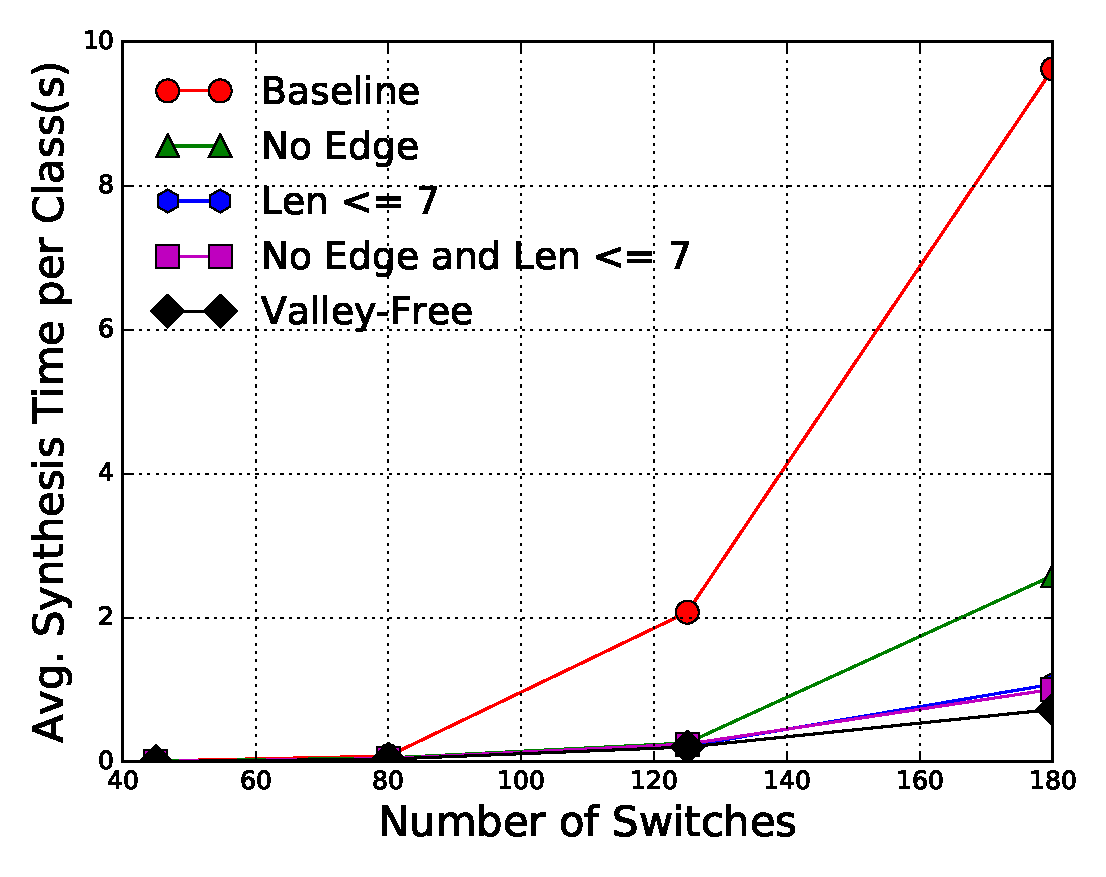
\includegraphics[width=0.65\columnwidth]{figures/isolationTopology.eps}
 	\compactcaption{Average synthesis time per packet class versus topology size for isolation workloads 
 		w/o different tactics with the ratio of packet classes to number of edge-aggregate links 0.25.}
 	\vspace{0.5cm}
 	\label{fig:tactic-topo}
 \end{figure}
 
\noindent {\bf Effect of Topology Size}: 
In \Cref{fig:tactic-topo},
 we evaluate the performance of different tactics for different topology sizes. There is a
 significant reduction in synthesis time for each tactic when compared to the baseline synthesis.
 The performance of each tactic is directly related to the reduction of the search space: more
 restrictive tactics have lower synthesis times. 
  Using the $length \leq 7$ tactic and ``no edge" tactic, \Name synthesizes forwarding rules for 20 tenants of group-size 5 in 100 seconds in a 180 switch
 topology (9$\times$ speedup over synthesis without tactics).
  
 \noindent{\bf Isolation with Link Capacity Policies}: A similar setup
 with additional link capacity constraints for 10 links is evaluated
 using the no edge tactic, and we get a best-case 14$\times$
 improvement over baseline synthesis. 
 Tactics can provide a considerable improvement
 over the baseline performance as illustrated by these experiments,
 and demonstrate the viability of synthesis approach of \Name to
 real-world networks.
 
\subsection{Divide-and-Conquer (DC) Synthesis Performance} \label{sec:optimisticeval} 
To evaluate the divide-and-conquer (DC) synthesis procedure, we
perform 100 runs of DC and non-DC synthesis 
(with the no edge tactic in both cases) on isolation
workloads with varying number of tenants and different group sizes
used in \secref{sec:baselineeval}. We compute the
speedup (time of non-DC synthesis/time of DC synthesis) and plot its
cumulative frequency distribution in \Cref{fig:dcsyn-cdf} to quantify
the benefits of DC synthesis. For more than 80\% of the
workloads, divide-and-conquer offers better or comparable
performance to non-DC synthesis, achieving a speedup of
2$\times$ for nearly 40\% of the workloads. For 20\% of the workloads,
divide-and-conquer performs worse than the non-DC approach,
especially for workloads with tenant group size 1 due to
greater number of recovery attempts. 

%  \aditya{How does this compare to ground up resynthesis? Without a comparison it is not clear minimal repair is useful!}

\minisection{Summary} The key points of our evaluation are:
1) For a representative tenant-group size of 10 in a 80 switch
  fat-tree, the baseline synthesis performance for synthesizing the
  forwarding rules for 1 to 8 tenants with complete tenant-isolation
  is in 0.1-2000s.
2) Operator policies like optimization objectives for TE and  
   network repair is more expensive than synthesis without
   objectives.
3) Tactics provide considerable speedup over the
        baseline synthesis.  We can
        synthesize the above workloads in 0.1-300s using the no edge
        tactic, and under 12s using the valley-free routing tactic.
4) \Name can further benefit from 
        divide-and-conquer (DC) synthesis, which provides a 2.0$\times$ speed-up
        over non-DC synthesis in 40\% of the workloads, in
        addition to the tactic improvements.
 
\section{Related \& Future Work} \label{sec:relatedwork}
\textbf{One Big Switch:} Kang et. al~\cite{oneswitch} tackle a 
similar problem of flow policy
enforcement. However their end-point policies deal with simple
reachability. Their rule placement algorithm takes the path of the
flow in the network  (called the routing policy) as an input. %  and place rules
% on this path to enforce the endpoint policy and taking in
% consideration switch table constraints
\Name supports policies like traffic isolation, 
for which it cannot determine the path of the flow
beforehand. % Our solution can support enforcement of policies which
% require different routing policies.
Zhang et. al~\cite{distfirewall} build on the "one big switch"  
abstraction~\cite{oneswitch} to optimize for the specific case of
distributed firewall policy enforcement using ILP.  PGA~\cite{pga} provides
a graph-level abstraction for specifying network policies like ACLs and
middlebox service chaining. However, PGA abstracts the underlying
network as "one big switch" and cannot be used to compose policies like
tenant isolation or traffic engineering.

 \noindent {\bf Controller synthesis:}
 Program synthesis has
 seen limited applications to SDN controllers~\cite{netegg,decentralize}.
These systems synthesize the
 behavior of individual switches (e.g., learning switches or
 firewalls); furthermore, these techniques apply to networks
 operating in a reactive mode (where the first packet of a connection
 is processed by the controller to determine the actions to
 employ). Such switch-centric approaches are too constraining and
 cannot be applied to realize network-wide objectives considered 
 in \name.
 
\noindent {\bf Policy languages:}
The closest approaches to ours are Merlin~\cite{merlin} and
NetGen~\cite{netgen}.  In Merlin data planes that adhere to policies
expressed using regular expressions are synthesized by first
intersecting the topology with the regular expressions appearing in
the policies and then encoding reachability in the intersected graph
using mixed integer linear programming (ILP).
%Unlike \Name, 
Merlin can support traffic engineering and load distribution. 
However, in its current iteration, 
Merlin's language does not support isolation policies, but we believe
that it could be extended to support them.  
%We cannot evaluate the
%performance impact of this extension, however.  
A more prominent
difference arises with unordered waypoint policies: expressing a
policy including a waypoint set $W$ of size $k$ requires a regular
expression of size exponential in $k$ as all the possible permutations
of the elements of $W$ must be considered. This fact clearly impacts the performance of
the Merlin's compiler that would have to generate a mixed ILP with a
large number of variables.  In \Name this is not the case as waypoints
can be encoded with polynomially many constraints.  While this does
not affect the theoretical complexity, our compiler does not incur
an a-priori exponential blow-up and it rather relies on the power
of SMT solvers to guide the search.  This is one of the main aspects
behind our decision of not using regular expressions to express
policies.  \Name uses a restricted form of regular expressions as 
tactics that leverage the network topology.  While in Merlin
regular expressions \emph{increase} the number of constraints
generated by the compiler, tactics \emph{decrease}
the number of generated constraints therefore speeding up the search.
To the best of our knowledge, this is the first use of constraints
that leverages the topology structure to simplify the search.

In NetGen, network updates that adhere to policies expressed using
regular expressions are synthesized using SMT solvers.  Given a
specification which mentions the packet classes, the old path, and the
new path, NetGen solves the network change problem using an SMT solver.
Due to the use of regular expressions NetGen also suffers the
limitations we just discussed for Merlin.  Interestingly, NetGen uses
a specific encoding of regular expressions based on uninterpreted
functions that helps reduce the number of constraints. While this
encoding is fast when updating a single path, we do not see a way to
extend it to our global synthesis setting.  A crucial aspect of NetGen
is that in its problem formulation each path can be synthesized
independently and without affecting the other already synthesized
paths.  This is not the case when supporting isolation policies: if an
old path needs to be moved to satisfy a new policy (e.g., because a
link is under maintenance), re-synthesizing such a path can require
re-synthesizing other paths. 
% \loris{we can have a small example of  this in appendix.}

% \noindent
% {\bf Synthesis for SDN:}
% Program synthesis has been actively applied in SDN for synthesizing the controller. Padon et. al in \cite{decentralize} try to synthesize
% local forwarding rules for a single switch based on a reactive
% forwarding policy.  NetEgg \cite{netegg} synthesizes the forwarding
% policy of a switch using examples of how the switch should function
% when it receives packets. These works deal with synthesis of
% forwarding behaviour of switches, and cannot be extended to satisfy
% network-wide policies.
Synthesis has been also used for generating consistent network
updates~\cite{updates, customconsistency}. But this problem is orthogonal to 
policy enforcement in \Name.

% Write about PGA, NetGen, and efficient update synthesis.

\noindent
{\bf Future directions:}
\Name has support for single-path traffic engineering, however in
practice, traffic is split in variable proportions along different 
paths for effective traffic engineering. One of the future 
directions of research is to extend the functionality of Genesis
to support fine-grained traffic engineering. Also, the performance
of SMT solvers with optimization objectives is quite slow, and calls for 
domain-specific techniques to speed up the synthesis. Also, datacenter
networks are highly symmetrical, and this symmetry can be leveraged
to speed up synthesis (similar to the work of Plotkin et. al~\cite{symmetry} to
speed up network verification using symmetry). The main challenges of
using symmetry in synthesis is considering two aspects of symmetry: network
symmetry and policy symmetry. Also, our treatment of resilience synthesis
is preliminary and future work will be geared towards synthesizing resilient
forwarding planes incorporating capacity constraints and traffic engineering.
 

\section{Conclusion}

We presented \Name, a general and extensible network management system
for enterprise-scale multi-tenant datacenter networks. It allows
rich policies to be specified declaratively. It leverages
the formal reasoning foundations of constraint solving together with
fast SMT solvers to synthesize data plane configuration from high
level policies. This abstracts away the difficult of programming or
configuring individual switches. \Name incorporates novel ideas to
speed up synthesis, leveraging the hierarchical nature of datacenter
network topologies and the structure of the interaction between
tenants' policies. These optimizations help \Name synthesize policies
for realistic settings in a few seconds, making it pratical to use in
network management.

%   Operators in multi-tenant cloud data centers require support for
%   diverse and complex end-to-end policies like reachability, middlebox
%   traversals, isolation, and network resource management. We present
%   \Name, a network management system which allows these policies to be
%   specified in a declarative manner without explicitly programming the
%   data-plane behavior.  \name tackles the problem of enforcing the
%   policies by synthesizing switch forwarding tables. In doing so, it
%   uses the formal reasoning foundations of constraint solving in
%   combination with fast off-the-shelf SMT solvers.  To improve
%   synthesis performance, \Name incorporates a novel search strategy that
%   uses regular expressions to specify properties that leverage the
%   structure of datacenter networks,
% %topologies to specify properties of the path 
%   and a heuristic synthesis procedure which exploits the structure of
%   policy interactions.  Experiments demonstrate the performance of
%   \Name with different workloads on real-world topologies. Overall,
%   the approach used by \Name is general and instrumental to building a
%   comprehensive network management system.



%\category{CR-number}{subcategory}{third-level}
%
%% general terms are not compulsory anymore,
%% you may leave them out
%\terms
%term1, term2
%
%\keywords
%keyword1, keyword2


%\acks
%
%Acknowledgments, if needed.

% We recommend abbrvnat bibliography style.

\bibliographystyle{abbrvnat}

% The bibliography should be embedded for final submission.
\bibliography{references}
\iffull
 \appendix
 \section{Proofs of NP-hardness} \label{sec:np}
 \subsection{Enforcement of Isolation Policies} \label{sec:isolationNP}
 Given a undirected graph $T=\{S,L\}$ which represents the switch topology denoted in \cref{fig:swtopo} and undirected graph $P =\{R,I\}$ which represents the policy graph. Every vertex $r \in R$ is a reachability policy : $s >> d$ and each edge $i \in I$ which connects vertices $r1$ and $r2$ mean that the paths of $r1$ and $r2$ are isolated from each other. 
 \begin{figure}[H] 
 	\centering
 	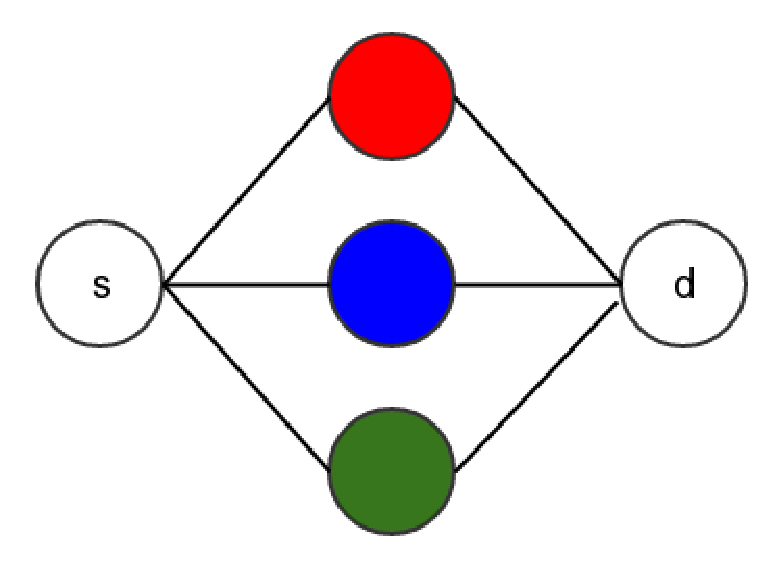
\includegraphics[width=0.7\columnwidth]{figures/color_topo.eps}
 	\caption{The switch topology $T$. All circles represent switches and all reachability policies are $s$ to $d$}
 	\label{fig:swtopo}
 \end{figure}
The solution to policy enforcement will be such that each reachability policy $r \in R$ from $s >> d$ will traverse through one of the colored switches $\{red$, $blue$, $green\}$. Color the vertices $R$ with the switch the path traverses through. If two vertices are connected by an edge in $I$, those flows would be isolated, and thus, will not have the same color. Thus, the problem reduces to finding a 3-graph coloring for the graph which is NP-complete. Thus, the enforcement of isolation policies is NP-complete. 
 
 In genral, k-coloring (for k > 2) is NP-complete and k-coloring problem reduces into a policy enforcement problem in a switch topology with k paths from source to destination, and thus, isolation policy enforcement is NP-complete. 
Similarly, The Hamiltonian Path problem can be reduced to an unordered waypoint policy, and thus, finding a path with unordered waypoints is NP-complete. The proof for this is omitted in this paper. 
 
% \subsection{Enforcement of Waypoint Policies}
% Given a undirected graph $G={V,E}$. Let us assume there exists an polynomial-time algorithm to compute the reachability paths satisfying the policies of the following types on the graph : \\
% \begin{itemize} 
% 	\item \textbf{P1} : $v_1 >> v_2 \Rightarrow$ There exists a path from $v_1$ to $v_2$ satisfying all input policies. A property of the path is that it does not have repeat a vertex (no forwarding loops).
% 	\item \textbf{P2} : $v_1 >> W >> v_2 \Rightarrow$ The path from $v_1$ to $v_2$  should pass through the vertices in the set $W$ in any order, without repeating a vertex.
% \end{itemize}
% \textbf{Reduction of Hamiltonian Cycle Problem} : Given a undirected graph $G={V,E}$, find $v \in V$ such that the degree of $v$ is the minimum in the graph (Will work for any vertex actually). If a Hamiltonian cycle is present in the graph, it will have the vertex $v$ in the cycle, and one of the edges from $v$.  \\
% Lets take a $n \in Neighbours(v)$. Let the input policies to our algorithm be : 
% \begin{itemize}
% 	\item \textbf{P4} : $v >> W >> n$ where $W = V - \{v,n\} $ 
% \end{itemize}
%P4 cimputes a simple path from $v$ to $n$ which passes through all the other vertices in the graph which is the Hamiltonian path problem. Since computing the Hamiltonian path is NP-hard, the problem of path computation for the waypoint policies as specified is NP-hard. 
\fi

\end{document}
